\documentclass[12pt]{article}

\usepackage[T1]{fontenc}
\usepackage[utf8]{inputenc}
\usepackage{fvextra}
\usepackage{csquotes}
\usepackage[czech]{babel}
\usepackage{caption}
\usepackage{geometry}
\usepackage{graphicx}
\usepackage{amsmath}
\usepackage{amssymb}
\usepackage{minted}
\usepackage{tocbibind}
\usepackage{parskip}
\usepackage{titlesec}
\usepackage[style=ieee]{biblatex}

\setlength{\parskip}{\baselineskip}
\setlength{\parindent}{2em}

\setcounter{tocdepth}{3}

\makeatletter
\renewcommand\tableofcontents{%
	\@starttoc{toc}%
}
\makeatother
\makeatletter
\renewcommand\listoffigures{%
        \@starttoc{lof}%
}
\makeatother

\addbibresource{bibliography.bib}

\captionsetup{font=small}
\usemintedstyle{vs}

\title{Kedarium}
\author{Robin Patrik Sloup}

\newboolean{isSOC}
\setboolean{isSOC}{true}

\begin{document}
\ifthenelse{\boolean{isSOC}}{
    \begin{titlepage}
    \begin{center}
        {\Large \textbf{STŘEDOŠKOLSKÁ ODBORNÁ ČINNOST} \par}
        \textbf{Obor č. 18: Informatika}
    \end{center}
    \vspace*{\fill}
    \begin{center} 
        {\Large \textbf{Kedarium, Grafický Engine}\par}
    \end{center}
    \vspace*{\fill}
    \begin{center}
        \begin{minipage}[t]{0.5\textwidth}
            \textbf{Robin Patrik Sloup}\\
            \textbf{Plzeňský kraj}
        \end{minipage}%
        \begin{minipage}[t]{0.5\textwidth}
            \raggedleft
            \break
            \textbf{Rokycany 2024}
        \end{minipage}
    \end{center}
    \thispagestyle{empty}
    \pagebreak
    \begin{center}
        {\Large \textbf{STŘEDOŠKOLSKÁ ODBORNÁ ČINNOST} \par}
        \textbf{Obor č. 18: Informatika}
    \end{center}
    \vspace*{\fill}
    \begin{center} 
        {\Large \textbf{Kedarium, Grafický Engine}\par}
        \vspace{0.3cm}
        {\Large \textbf{Kedarium, Graphics Engine}\par}
    \end{center}
    \vspace*{\fill}
    \textbf{Autoři}: Robin Patrik Sloup \\
    \textbf{Škola}: Gymnázium a SOŠ Rokycany, Mládežníků 1115/II, 337 01 Rokycany\\
    \textbf{Kraj}: Plzeňský kraj \\
    \textbf{Konzultant}: Mgr. Jitka Fürbacherová \\

    \noindent Rokycany 2024
    \thispagestyle{empty}
\end{titlepage}

}{
    \begin{titlepage}
    \begin{center}
        {\Large Gymnázium a Střední Odborná Škola\par}
        ul. Mládežníků 1115, Rokycany
    \end{center}
    \begin{center}
        \vspace{1cm}
        
\includegraphics[height=3cm]{images/school-logo.png}\\
    \end{center}
    \vspace*{\fill}
    \begin{center} 
        {\Huge \textbf{Kedarium,\\Grafický Engine}\par}
        \vspace{0.3cm}
        {\Large Maturitní Práce\par}
        \vspace{1.5cm}
    \end{center}
    \vspace*{\fill}
    \begin{center}
        \begin{minipage}[t]{0.45\textwidth}
            \centering
            \textbf{Autor Práce:}\\
            Robin Patrik Sloup
        \end{minipage}%
        \begin{minipage}[t]{0.45\textwidth}
            \centering
            \textbf{Vedoucí Práce:}\\
            Mgr. Jitka Fürbacherová
        \end{minipage}
    \end{center}
    \vspace{2cm}
    \begin{center}
        Rokycany 2024
    \end{center}\textbf{}
    \thispagestyle{empty}
\end{titlepage}

}
\ifthenelse{\boolean{isSOC}}{
    \setcounter{page}{3}
}{
    \setcounter{page}{2}
}

\ifthenelse{\boolean{isSOC}}{
    \section*{Prohlášení}

Prohlašuji, že jsem svou práci SOČ vypracoval samostatně a použil jsem pouze prameny a literaturu uvedené v seznamu bibliografických záznamů.

\noindent Prohlašuji, že tištěná verze a elektronická verze soutěžní práce SOČ jsou shodné. 

\noindent Nemám závažný důvod proti zpřístupňování této práce v souladu se zákonem č. 121/2000 Sb., o právu autorském, o právech souvisejících s právem autorským a o změně některých zákonů (autorský zákon) ve znění pozdějších předpisů. 

\vspace{24pt}
\noindent
V Rokycanech dne 20. 3. 2024 — Robin Patrik Sloup
\thispagestyle{empty}
\pagebreak

}{
    \section*{Prohlášení}

Prohlašuji, že jsem maturitní práci s názvem „Kedarium, Grafický Engine“ vypracoval samostatně pod vedením Mgr. Jitky Fürbacherové a uvedl v seznamu literatury všechny použité literární a odborné
zdroje. Dále prohlašuji, že citace použitých pramenů je úplná a že jsem v práci neporušil
autorská práva (ve smyslu zákona č. 121/2000 Sb. O právu autorském, o právech souvisejících
s právem autorským).

\vspace{24pt}
\noindent
V Rokycanech dne 20. 3. 2024
\thispagestyle{empty}
\pagebreak

}
\section*{Poděkování}

Mé poděkování patří Mgr. Jitce Fürbacherové za odborné vedení, ochotu a trpělivost, kterou mi v průběhu zpracování této práce věnovala. Dále děkuji Jakubu Trnčákovi za pomoc při testování práce na systému MacOS.

\thispagestyle{empty}
\pagebreak

\section*{Anotace}

Práce řeší tvorbu grafického enginu v programovacím jazyce C++ s využitím grafického rozhraní OpenGL. Abstrahuje grafické a matematické komponenty do vlastních tříd, přičemž využívá paradigmatu objektového programování. Jedná se o střední cestu mezi tvorbou enginu vlastního a využitím komerčního řešení. Soustředí se na implementaci grafiky a řešení logiky nechává na starost programátoru.

\subsubsection*{Klíčová slova}

C++, OpenGL, grafické rozhraní, abstrakce, OOP, shadery, světlo, lineární algebra, modely, textury

\section*{Annotation}

The work addresses the creation of a graphics engine in the C++ programming language using the OpenGL graphics interface. It abstracts graphical and mathematical components into its own classes, utilizing the object-oriented programming paradigm. It represents a middle ground between creating a custom engine and utilizing a commercial solution. It focuses on the implementation of graphics, leaving the solution of logic to the programmer's responsibility.

\subsubsection*{Keywords}

C++, OpenGL, graphics interface, abstraction, OOP, shaders, lighting, linear algebra, models, textures

\thispagestyle{empty}
\pagebreak


\section*{Obsah}
\tableofcontents
\pagebreak

\pagebreak

\section{Úvod}

Tato práce se zabývá problematikou tvorby grafického enginu — vývojové knihovny pro vývoj grafických aplikací, s využitím pouze základních, externích knihoven, díky kterému může programátor tvořit různé 3D scény a dodat jim svou vlastní funkcionalitu.

Pro tvorbu her či animací se často využívají komerční nástroje, které disponují širokou škálou možností a funkcí, pro tvorbu dechberoucích titulů a děl. Nevýhodou je, že zřídkakdy všechny tyto funkce vyžadujeme. Moderní herní enginy sice optimalizují výsledek, který jde do produkce, vždy ale bude obsahovat více kódu, než je třeba, a tak náš výsledný produkt nebude tak výkonný, jak by ve skutečnosti mohl být. Jedním z řešení je napsat si pro naší hru nebo projekt engine vlastní. Tímto způsobem můžeme optimalizovat každý aspekt, který musíme při tvorbě grafických programů zvážit a vytvořit tak dílo podle našich představ.

Pokud bychom pro každý grafický program, který tvoříme, psali ale engine vlastní, brzy bychom z časových důvodů moc takovýchto programů nevytvořili. Cílem této práce je vytvořit engine, který abstrahuje složitosti spojené s prací s grafickým rozhraním a zároveň nabízí výkonné řešení. Engine by měl být schopen abstrahovat základní koncepty, které jsou společné ve většině grafických projektech, na takovou úroveň, aby uživatel enginu věděl, co se v jeho programu děje a přitom se nemusel zabývat problematikou, která není pro jeho program specifická. Pod těmito koncepty si představme správu a tvorbu okna, získávání vstupu z klávesnice, pohyb v prostoru, operace s prostorem, načítání modelů ze souborů nebo např. simulace světla.

Engine by měl také být dostatečně modulární, díky čemuž nemusí být programátor závislý na celé jeho funkcionalitě, nýbrž na konkrétních, atomických částech. Pokud problém vývojáře vyžaduje jinou variantu, jak načítat modely těles, ale stále chce využít dostupné části enginu, nemá v cestě žádnou překážku pro realizaci vlastní části řešení. Je žádoucí, aby jednotlivé části práce šly využívat samostatně.

Konzistence je klíčem k úspěchu; engine by měl býti ve svém fungování a názvosloví celistvý. Programátor tak vždy bude chápat, co daná funkce vykonává, aniž by si musel dohledávat implementaci v samotném enginu. Moduly a funkce enginu musí býti konzistentně komentovány, pro jednoduchou a intuitivní práci s nimi. Díky tomuto faktoru pak mohou dílčí části tvořit fungující celek. Po seznámení s enginem by měl vývojář být schopný odvodit, co má daný modul či jeho část na starost i bez předchozích zkušeností a referencí.

Díky abstrakcím můžeme integrovat prvky enginu do vícero projektů bez znalosti implementace; nesmí se to však s abstrakcí přehánět. V momentě, kdy je logika příliš zobecněna, třetí osoba ztrácí pojem o tom, co se v jejím programu děje. Pak nemůžeme tvrdit, že engine usnadňuje práci — abstrakce se musí přizpůsobit vývojáři, nikoliv naopak. Engine se musí snažit o zjednodušení a srozumitelnost zároveň.

Engine si dává za cíl tyto jednotlivé podmínky splňovat a nabízet tak vývojářům možnost, jak učinit jejich práci při vývoji snazší, nerepetetivní a efektivní. Má býti střední cestou, mezi používáním komerčních řešení a tvořením všech dílů stavebnice od základu.

Následuje kapitola analýza, kde problematiku přiblížím více a rozvedu koncepty potřebné pro pochopení. Další kapitola se zabývá samotnou implementací a řešení problému, společně s ukázkami v kódu. Testování je věnována samotná, následné kapitola. Součástí práce je i uživatelský manuál pro spuštění a sestavení projektu vytvořeného tímto enginem.

\pagebreak

\section{Analýza}

Pro realizaci práce je nutné správně zvolit grafické rozhraní, programovací jazyk a chápat základní grafické koncepty. V této kapitole budou představeny různé nástroje pro řešení našeho problému a následně bude provedena diskuze na téma, jaké jsou klady a zápory daných řešení a samotné finální volby.

Na konci této kapitoly se zaměřím na popis matematických konceptů, jež budou pro vhodné řešení využity. Tyto koncepty se využívají primárně pro práci s prostorem. Nalézají ale i jiná využití — více o nich si povíme v kapitole implementace.

\subsection{Volba grafického rozhraní} \label{g_interface}

Grafické rozhraní můžeme považovat za střední bod mezi našimi instrukcemi v programu a samotnou grafickou kartou, která má na starost vykreslování grafiky v daném zařízení. Grafické karty mohou mít různé výrobce, samotný výrobce distribuuje různé modely, řady, verze, apod., a tedy odlišný způsob, jak danou instrukci musí karta vykonat. Ne každý grafický čip umožňuje vykonat danou instrukci, popřípadě ne na stejné úrovni.

Rozhraní pro programování aplikací, též API (Application Programing Interface), mají za úkol abstrahovat hardware či technologické rozdíly daného komponentu nebo systému a zobecnit tak práci s ním. Vývojář tedy nemusí přemýšlet nad implementací pro různé typy systémů, ale dostává standard, díky kterému může komunikovat se širokou škálou komponentů.

Grafické rozhraní představuje specifickou kategorii uživatelského rozhraní, jež nám umožňuje efektivně využívat možnosti grafických karet a zajišťuje jejich bezproblémovou komunikaci napříč různou hardwarovou výbavou. Potřebuji-li provést instrukci s grafickou kartou od společnosti NVIDIA, bez problému mohu funkcionalitu replikovat i na grafické kartě společnosti AMD. Nyní je důležité zvolit vhodné rozhraní pro náš projekt.

Několik nejběžněji používaných grafických rozhraní zahrnuje OpenGL \cite{opengl}, Vulkan \cite{vulkan}, DirectX \cite{directx}, WebGPU \cite{webgpu} a OpenGL ES \cite{opengles}. Začal jsem tím, že jsem eliminoval rozhraní, která nejsou určena pro řešení mého problému. Nebudu se zabývat jejich výhodami, či nevýhodami, neb pro tuto práci nejsou vhodné. Například, WebGPU je primárně určeno pro práci ve webových prohlížečích, kde umožňuje interakci s grafickou kartou pro výpočty a vykreslování v prohlížeči. Dále jsem eliminoval OpenGL ES. Toto API je cíleno pro embedded zařízení a mobilní systémy. Příkladem těchto zařízení mohou být konzole, mobilní telefony nebo chytrá vozidla. Více informací o tomto API lze nalézt na stránkách konsorcia Khronos Group \cite{khronos}. Jedná se o neziskové konsorcium, které vyvíjí standardy pro grafiku, virtuální a rozšířenou realitu nebo strojové učení. Některé standardy a specifikace, které vyvíjí toto konsorcium jsou: OpenGL, glTF, OpenCL a OpenXR.

Měl jsem tedy tři volby; OpenGL, DirectX a Vulkan. OpenGL široce rozšířený standard, který je téměř všude podporován. Poskytuje výkonné API s velkou komunitou a problémy, které s ním mohou vzniknout, jsou často již vyřešeny. Velkou výhodou je i multiplatformnost rozhraní. Ze stinné stránky si OpenGL prošlo mnoha změnami a můžeme tak nalézt spoustu zdrojů a materiálů, které jsou zastaralé. Navíc je API samo považováno za zastaralé s doporučením přechodu na Vulkan. Za nevýhodu lze považovat i to, že OpenGL nemá na starost jedna entita ale konsorcium; nemůže tedy existovat oficiální podpora.

Samotný Vulkan má stejně jako OpenGL na starost konsorcium Khronos Group. Umožňuje velmi detailní úpravy operací, které vedou k vykreslení grafiky na obrazovku. Pro vývojáře, kteří chtějí mít skvěle optimalizovaný engine, se kterým lze tvořit moderní hry nebo VR produkty, je toto API skvělá volba. Snaží se nezatěžovat procesor zařízení a směrovat práci grafické kartě. Také má velmi dobrou podporu pro multi-threading — schopnost souběžně vykonávat více operací naráz. Nevýhodou je, že se jedná o poměrně komplexní API. Začít s Vulkanem je složitější, než u většiny jiných API, kód aplikací je delší a tvorba prototypů a menších řešení, které nepotřebují využívat všech jeho funkcí, se tak značně zpomaluje.

Jako poslední představím DirectX. DirectX je kolekce proprietárních rozhraní vyvinutých společností Microsoft. Samotný grafický komponent DirectX se nazývá Direct3D. Toto API je primárně určeno pro hry. Snaží se o zpětnou kompatibilitu mezi verzemi a má rozsáhlou dokumentaci, spravovanou společností Microsoft. Má výbornou podporu pro systém Windows, protože je pro tento systém určen. Podpora dalších platforem ale není tak kvalitní. Někomu by také mohlo vadit, že vývoj API je přímo závislý na společnosti Microsoft a s vydáními se musí čekat právě na ni.

Můj cíl je vytvořit multiplatformní grafický engine, čemuž ne zcela vyhovuje API DirectX. Rozhodování je tedy mezi Vulkanem a OpenGL. Práci tvořím sám a tvorba řešení a implementace by s Vulkanem trvala značně déle. Dále také nevyžaduji pokročilé funkce, které Vulkan nabízí. Mou finální volbou se tedy stává OpenGL. Ačkoliv je považováno za zastaralé, nabízí i moderní verze, které se i dnes používají nejen v herním průmyslu. Má rozsáhlou komunitu a podporu, proto ho i přes zdánlivou zastaralost považuji za vhodné řešení.

\subsection{OpenGL} \label{opengl}

OpenGL je standard, který nám dává možnost interagovat s daty, vykreslováním a zpracováním grafiky, bez ohledu na hardware zařízení. Slouží čistě pro práci s grafickou kartou a neřeší např. tvorbu okna, získání vstupu z klávesnice, načítání obrázků nebo načítání modelů. První verzi OpenGL vytvořila americká firma Silicon
Graphics Computer Systems v roce 1994. Nachází využití v mnoha průmyslech, ať už herním, věděckém nebo zdravotním. Funguje na bázi grafické pipeline — seřazený postup operací, který nám ze vstupních dat tvoří vizualizaci na obrazovce. Grafickou pipeline bychom mohli přirovnat k výrobní lince, kde každý její segment má pevně daný úkol, a na konci vzniká výsledný produkt.\cite{Shreiner_2013}

\vspace{0.5cm}
\begin{figure}[h]
    \centering
    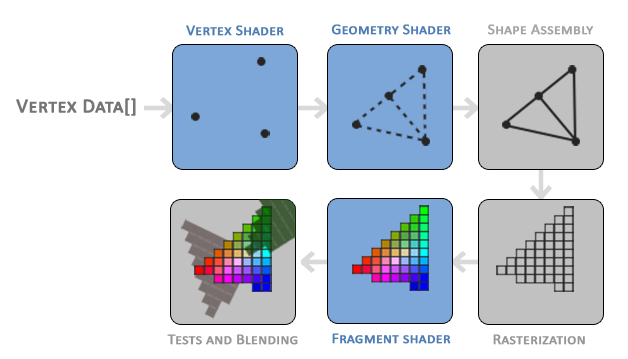
\includegraphics[width=10cm]{images/opengl_pipeline.png}
    \caption[Grafická pipeline OpenGL]{Grafická pipeline OpenGL \cite{pipeline_img}}
    \label{fig:Grafická pipeline OpenGL}
\end{figure}
\pagebreak

Jak vidíme na Obrázku \ref{fig:Grafická pipeline OpenGL}, na začátku do pipeline zasíláme data o vrcholech. Tato data mohou obsahovat informaci o pozici vrcholu, jeho barvu, jeho normálový vektor, apod. Následně vektorový shader těmto datům dodá význam. Shader je malý program, který má za úkol přeměnit vstup na jiný výstup.\cite{lopgl_shaders} Díky vrcholovému shaderu víme, co jaká data reprezentují. Pipeline pokračuje geometrickým shaderem, který nemusíme implementovat. Uvnitř něj můžeme upravit zaslaná data o vrcholech, vrcholy odebrat nebo tvořit nové.\cite{lopgl_geometry_shader}

Dalším krokem je tvorba tvarů. V této fázi OpenGL přemění skupinu vrcholů na jednotlivé trojúhelníky. Trojúhelníky jsou vhodný útvar, neboť tři vrcholy jsou nejmenší nutný počet vrcholů pro definování roviny a dají se s nimi aproximovat všechny další tvary a tělesa. Nyní grafická pipeline provede proces rasterizace, který, jak vidíme na Obrázku \ref{fig:Grafická pipeline OpenGL}, přemění trojúhelníky na souřadnice na obrazovce. Pak přichází na řadu fragmentový shader. Ten může vrcholu přiřadit barvu, pixel z obrázku nebo na něj např. aplikovat světlo. Jako poslední krok spustí OpenGL několik testů. Může například zjistit, který objekt je vůči nám blíž a ten vykreslit, podobně, jako kdybychom skládali obrázky na papíru na sebe. Také se v tomto bodě zpracuje průhlednost ploch.

\subsection{Volba programovacího jazyka}

Velmi důležité je i správně zvolit programovací jazyk pro implementaci řešení. Musíme zvážit více faktorů jako dostupnost knihoven — souhrn již napsaného kódu pro daný účel (např. knihovna pro tvorbu a správu okna a jeho vstupů), výkon jazyka či jeho funkce. Pro řešení jsem chtěl použít jazyk, se kterým jsem se již setkal a mám s ním zkušenosti, aby mě neznalost daného jazyka nebrzdila či neomezovala při tvorbě programu. Rozhodoval jsem se mezi těmito jazyky: C, C++, Python a Java.

C \cite{kandr} je všestranný programovací jazyk, který v roce 1972 vytvořil Dennis Ritchie pro použití operačním systémem UNIX. Jedná se o nízkoúrovňový jazyk — programátor může ku příkladu přímo pracovat s pamětí počítače a tvořit vysoce optimalizované programy. Je to velmi rychlý a dodnes stále rozšířený jazyk. V tomto jazyce je napsaná spousta užitečných nástrojů, jako Git \cite{git}, Apache \cite{apache} nebo Linuxový \cite{linux} kernel. To, že je nízkoúrovňový, také ale znamená, že nepodporuje velké množství funkcí moderních programovacích jazyků a tvořit větší aplikace tímto jazykem by značně prodloužilo dobu vývoje a komplexitu kódu.

C++ \cite{cpp} bývá často považováno za nástupce C. Vytvořil ho Bjarne Stroustrup v roce 1979 a původně se jazyk jmenoval "C with classes". Dává si za cíl řešit problémy jazyka C, umožňuje psát kód různými paradigmaty — způsoby či schématy myšlení a snaží se také vytvořit nový pohled na psaní kódu. C++ je rychlý a flexibilní jazyk, který již v základu poskytuje velké množství funkcí. Tento jazyk umožňuje psaní nízkoúrovňového kódu a zároveň používání funkcí moderních jazyků. Nyní uvedu několik příkladů aplikací, které C++ využívají: Mozilla Firefox \cite{firefox}, Adobe Photoshop \cite{photoshop} či databáze MySQL \cite{mysql}. Nevýhodou C++ ale může být jeho složitost a rozsáhlost. Jazyk má spoustu standardů a často se stává, že projekty psané tímto jazykem používají svou vlastní část a implementaci jazyka. Člověku, který se s tímto jazykem nesetkal, bude trvat naučení se jazyka na pokročilou úroveň značně déle, než u jiných moderních a používaných jazyků.

Python \cite{python} se od C a C++ značně liší již v základu. Jedná se o jazyk interpretovaný, zatímco C a C++ jsou jazyky kompilované. To, že je Python interpretovaný, znamená, že se zdrojový kód převádí na strojový kód, kterému rozumí počítač, za chodu aplikace. U  kompilovaných jazyků se kód zpracuje naráz a vznikne nám spustitelná aplikace. Jedná se o velmi přizpůsobivý jazyk; nachází využití v grafice, zpracování dat, strojovém učení, v tvorbě desktopových aplikací a na spoustě dalších místech. Je dobře čitelný a dá se snadno naučit, proto je také často doporučován začínajícím programátorům. Také pro něj existuje velké množství knihoven, včetně knihoven pro práci s OpenGL. Jeho zásadní nevýhodou je ale výkon. Díky interpretaci kódu za chodu se stává poměrně pomalým. Oproti C (a to bez optimalizací) řeší Python většinu úkolů i 50x pomaleji. Pokud chceme psát optimalizovaný a výkonný kód, Python pravděpodobně není vhodná volba.

Jako poslední programovací jazyk jsem zvažoval jazyk Java \cite{java}. S tímto jazykem se mimo jiné setkávám i na škole, kde studuji. Jedná se o moderní, objektově orientovaný jazyk, který nabízí téměř bezkonkurenční podporu pro více platforem. Objektové programování \cite{oop} seskupuje atributy a chování do jednoho bloku, objektu, který vytváří šablona — třída. Tyto třídy můžou dále implementovat dědičnost. Řekněme, že mám třídu (šablonu) člověk. Ta může vytvořit objekt, který má parametry věk, jméno a bydliště. Také má svou funkcionalitu, může jíst, spát nebo studovat. Dědičná třídou by mohl být zaměstnanec, který má stejné atributy a chování jako třída člověk, mimo jiné má ale atribut plat a funkcionalitu pracování. Java je jazyk, který tento styl programování rozšířil a ovlivnil jím i další jazyky. Využívá technologii JVM (Java Virtual Machine)\cite{jvm}, díky které se její kód spouští na virtuálním hardware a není tak závislý na jeho fyzické implementaci. To umožňuje spouštět Java kód kdekoliv, kde JVM je. Díky spouštění skrze JVM ale nebývá tak rychlá jako standardní kompilované jazyky. Některým programátorům by také nemuselo vyhovovat, že se Java soustředí výhradně na objektově orientované paradigma. Při programování v Javě máme také poměrně omezené, jaké nízkoúrovňové funkcionality lze používat.

Nyní se pojďme zamyslet, jak pro práci zvolit vhodný jazyk. Úkolem práce je vytvořit grafický engine, který umí spravovat okno, získávat vstupy z počítače a pracovat s 3D prostorem. Grafický engine by měl být pokud možno co nejrychlejší, to znamená i volbu rychlého programovacího jazyka. Všechny zmíněné jazyky mají řadu knihoven pro interakci s API OpenGL a splňují tak základní požadavky enginu. Jako první jsem eliminoval programovací jazyk Python. Pro tvorbu enginu, který je rychlý a zároveň je schopný dostatečně abstrahovat OpenGL koncepty by použití Pythonu nebylo vhodné. Zbývalo mi tedy rozhodnout se mezi C, C++ a Javou. Jako další jsem odebral Javu, protože nemá tolik nízkoúrovňových funkcí jako C a C++. Zároveň mám v těchto jazycích i více zkušeností, než s jazykem Java. Dlouhou dobu jsem zvažoval, že pro realizaci práce zvolím jazyk C. Když jsem ale tvořil prototypy enginu, zjistil jsem, že vyvíjet tímto způsobem engine zabere poměrně velkou dobu, nebudu mít tolik možností abstrahování konceptů a změna logiky by znamenala přepsání většiny kódu.

Díky této zkušenosti jsem nakonec zvolil použití jazyka C++. Tento jazyk poskytuje možnost práce v objektově orientovaném stylu, což je vhodné pro abstrakci grafických konceptů do vlastních tříd, ale zároveň nabízí i práci s nízkoúrovňovými koncepty, jako např. operace s pamětí zařízení. Má také spoustu užitečných funkcí, které více přiblížím v kapitole, zabývající se implementací řešení.

\subsection{Grafické koncepty}

Pro implementaci je také nutné si atomizovat některé koncepty a shrnout si, k čemu slouží a jak je budeme moct využít. Vytvořil jsem si seznam těch, které je nutné dobře definovat, neboť na nich stojí základy celého programu. Jejich správná implementace je nutná pro fungování aplikace jako celku.

\subsubsection{Okno} \label{okno}

Okno je prvkem GUI (Graphical User Interface)\cite{gui}, grafického uživatelského rozhraní. Můžeme ho přirovnat k jakémusi inteligentnímu plátnu, které patří danému programu. Konkrétně v našem případě budeme na toto plátno vykreslovat grafiku. Samo okno může obsahovat další prvky uživatelského rozhraní, jako tlačítka, texty, zadávací pole a dalších mnoho elementů. Funkcionalita okna se liší na bázi jeho implementaci operačním systémem nebo jeho prostředím, můžeme však zobecnit funkce, které se mezi systémy téměř neliší. Okna lze minimalizovat (skrýt je), měnit jejich velikost, zavírat nebo s nimi vyplnit obrazovku. \cite{window}

\vspace{0.5cm}
\begin{figure}[h]
    \centering
    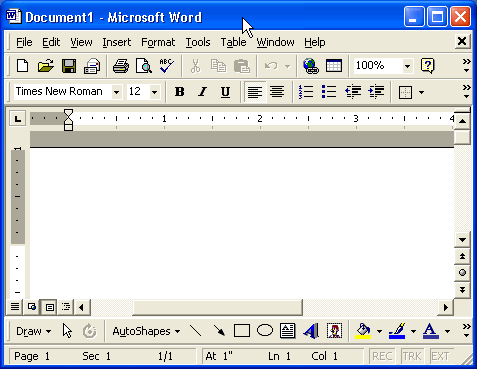
\includegraphics[width=10cm]{images/xp_window.png}
    \caption[Okno programu MS Word v operačním systému Windows XP]{Okno programu MS Word v operačním systému Windows XP \cite{xp_window}}
    \label{fig:Okno programu MS Word v operačním systému Windows XP}
\end{figure}

Na Obrázku \ref{fig:Okno programu MS Word v operačním systému Windows XP} můžeme vidět okno aplikace Microsoft Word \cite{word}, která běží na operačním systému Windows XP. Samotné okno má svůj titulek, který vidíme v horní modré liště. Na pravé straně se nacházejí tlačítka pro operace s oknem. Konkrétně Microsoft Word slouží pro tvorbu a úpravu dokumentů, má tedy i příslušné nástrojové lišty. Tvorba a správa okna je jedna z fundamentálních podmínek, pro vykreslování grafiky na obrazovku uživatele.

\subsubsection{Kamera}

Kameru si můžeme představit jako digitální oči programů pracujících s vykreslováním grafiky. Má svou pozici, směr pohledu a zorné pole — oblast, kterou můžeme pozorovat v daný moment. Může mít i další parametry, jako např. vzdálenost, do které kamera vidí. Nemusí pracovat jen s třírozměrným prostorem, můžeme mít kameru určenou pro plochu, která se často používá pro hry v pohledu z boku (např. Terraria \cite{terraria}) nebo pro vykreslování bokorysu (pohledu na objekt z boku) v technických programech. \cite{camera}

\vspace{0.5cm}
\begin{figure}[h]
    \centering
    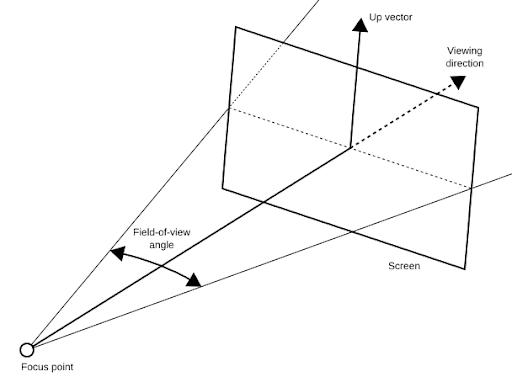
\includegraphics[width=14cm]{images/camera.png}
    \caption[Jednoduchý nákres fungování kamery]{Jednoduchý nákres fungování kamery \cite{camera_img}}
    \label{fig:Jednoduchý nákres fungování kamery}
\end{figure}

Jak vidíme na Obrázku \ref{fig:Jednoduchý nákres fungování kamery}, v závislosti na úhlu zorného pole, pozici a směru kamery můžeme ovlivnit, co se vykreslí uživateli na obrazovku. Kamery najdeme ve všech grafických hrách, technických programech či v modelovacích programech (např. v Blenderu \cite{blender}). Kvalitní implementace kamery a plynulých změn jejího stavu je podstatná pro kladnou uživatelskou zkušenost. Ku příkladu, kdyby se kamera při rotaci zasekávala nebo zkreslovala délky těles, nebude mít uživatel pocit, že se pohybuje realisticky působícím prostředím, ale spíše ne příliš kvalitní simulací prostoru. Kamera je jednoduchý koncept, který na první pohled nepůsobí jako elementární část programu. Musíme ale mít na paměti, že se jedná o koncept, se kterým uživatel interaguje většinu času — nekvalitní implementace uživateli neprodá kvalitní zážitek.

\subsubsection{Vertex Buffer Object}

Nyní zavedu grafický pojem, který je specifický pro naše vybrané grafické rozhraní, tedy OpenGL. VBO (Vertex Buffer Object) je buffer objekt, který se používá jako zdroj vrcholových dat. To je bez předchozího kontextu či znalostí téměř nic neříkající; pojďme si tedy tento pojem vysvětlit. Buffer objekt \cite{buffer_object} je kolekce dat, která má svůj specifický účel. Může například představovat informace o vrcholech (jednotlivých bodech těles) nebo informace o pixelech získaných z obrázku. \cite{vao_vbo_ebo}

\vspace{0.5cm}
\begin{figure}[h]
    \centering
    
\includegraphics[height=6cm]{images/vbo.png}
    \caption{Příklad VBO s daty}
    \label{fig:Příklad VBO s daty}
\end{figure}

Konkrétně VBO má na starost seskupovat data o vrcholech. Na Obrázku \ref{fig:Příklad VBO s daty} můžeme vidět čtverec, který se skládá ze čtyř vrcholů. Vidíme, že každý vrchol má svou pozici a svou barvu. Pod čtvercem vidíme seznam hodnot, který se skládá z osmi trojic. Konkrétně zde náleží každému vrcholu právě 2 trojice — pro jeho pozici a barvu. Tento význam dává hodnotám vývojář, OpenGL u VBO nerozlišuje, která hodnota znamená jaký atribut.

\subsubsection{Element Buffer Object}

S VBO úzce souvisí Element Buffer Object, zkráceně EBO. Ten seskupuje data o tom, jaké trojúhelníky tvořit z dat o vrcholech. Již jsem zmínil, že OpenGL používá pro vykreslování ploch a těles trojúhelníky. Chci-li vykreslit čtverec, musím k sobě přiložit 2 shodné, pravoúhlé trojúhelníky. To by ale znamenalo, že potřebuji mít definovaných 6 vrcholů, 3 pro každý trojúhelník. Představme si, že chci vykreslit krychli. Každý vrchol je zároveň součástí tří stran. Znamená to, že pro vykreslení jednoduché krychle potřebuji definovat 24 vrcholů, přesto že ji lze vyjádřit vrcholy osmi. \cite{vao_vbo_ebo}

\vspace{0.5cm}
\begin{figure}[h]
    \centering
    
\includegraphics[height=6cm]{images/ebo.png}
    \caption{Příklad EBO s daty}
    \label{fig:Příklad EBO s daty}
\end{figure}

Tuto problematiku řeší EBO, které nám udává, jak na bázi pořadí vrcholů ve VBO vykreslovat trojúhelníky. Použijeme stejný čtverec z příkladu k VBO a aplikujeme na něj tento princip. Čtverec popíšeme čtyřmi vrcholy a do EBO vložíme dvě trojice jenž popisují, jaké vrcholy trojúhelníky využívají. Na obrázku \ref{fig:Příklad EBO s daty} vidíme pořadí jednotlivých vrcholů a jak mohou data v EBO vypadat. Trojice $(0, 1, 2)$ vykreslí pravý dolní trojúhelník a trojice $(0, 2, 3)$ pak trojúhelník vlevo nahoře. Jedná se o malou ale efektivní optimalizaci, která v měřítku jednoho čtverce nepůsobí jako velká změna; většina detailních modelů má ale miliony trojúhelníků a tak optimalizace počtu potřebných vrcholů jedním z rozhodujících faktorů výkonu vykreslování našeho programu. Představme si EBO jako manuál ke skládání dat z VBO do jednoho celku pro naší grafickou kartu.

\subsubsection{Vertex Array Object}

Data v tento moment nemají pro OpenGL konkrétní význam; čte jen dlouhý seznam hodnot. Koncept, kterým můžeme OpenGL předat informace o datech vrcholů se nazývá VAO (Vertex Array Object). Podívejme se znovu na Obrázek \ref{fig:Příklad VBO s daty}, v sekci vysvětlující VBO. Můžeme data zobecnit a vytvořit si seznam informací o nich. Práce s VAO je v základu předání tohoto seznamu:

\begin{enumerate}
    \item Prvním komponentem je pozice.
    \item Pozice zabírá celkem 3 hodnoty.
    \item Pozice je reprezentována celými čísly.
    \item Mezi hodnotami není žádná mezera nebo jiná hodnota.
    \item Začátek další informace o pozici se opakuje po každých šesti hodnotách.
\end{enumerate}

Součástí popisu by pak mohlo být i to, kde může OpenGL najít barvy vrcholů, např. jako na Obrázku \ref{fig:Příklad VBO s daty}. Úkolem VAO je uchovávat hodnoty, společně s jejich formátem — popisem, jak jsou data rozsáhlá, kde je najít a o jaký druh hodnot se jedná. Nyní má OpenGL všechny informace, které potřebuje pro sestavení celku, dle našich potřeb. \cite{vao_vbo_ebo}

\subsubsection{Textura}

Textura je zpravidla dvourozměrný obrázek (v některých případech může mít dimenze jiné), který slouží pro přidání detailů objektu. Pokud by chtěl programátor vytvořit kamennou zeď, potřeboval by spoustu vrcholů, pro popsání jednotlivých výběžků, hrubosti povrchu či prasklin ve zdi. Texturu lze využít pro přidání detailů a dát tělesu více realistický vzhled. Také díky ní není potřeba přidávat více vrcholů a nedělat tak kompromisy na výkonu programu. Může se jednat o jakýkoliv obrázek, je ale poměrně důležité, aby byl čtvercový a jeho rozměry byly mocniny čísla 2, např. 16x16, 32x32, 128x128 nebo 1024x1024. Starší grafické karty mají problém s nečtvercovými formáty a také díky tomuto formátu může OpenGL aplikovat řadu optimalizací při práci s texturou. \cite{texture}

\vspace{0.5cm}
\begin{figure}[h]
    \centering
    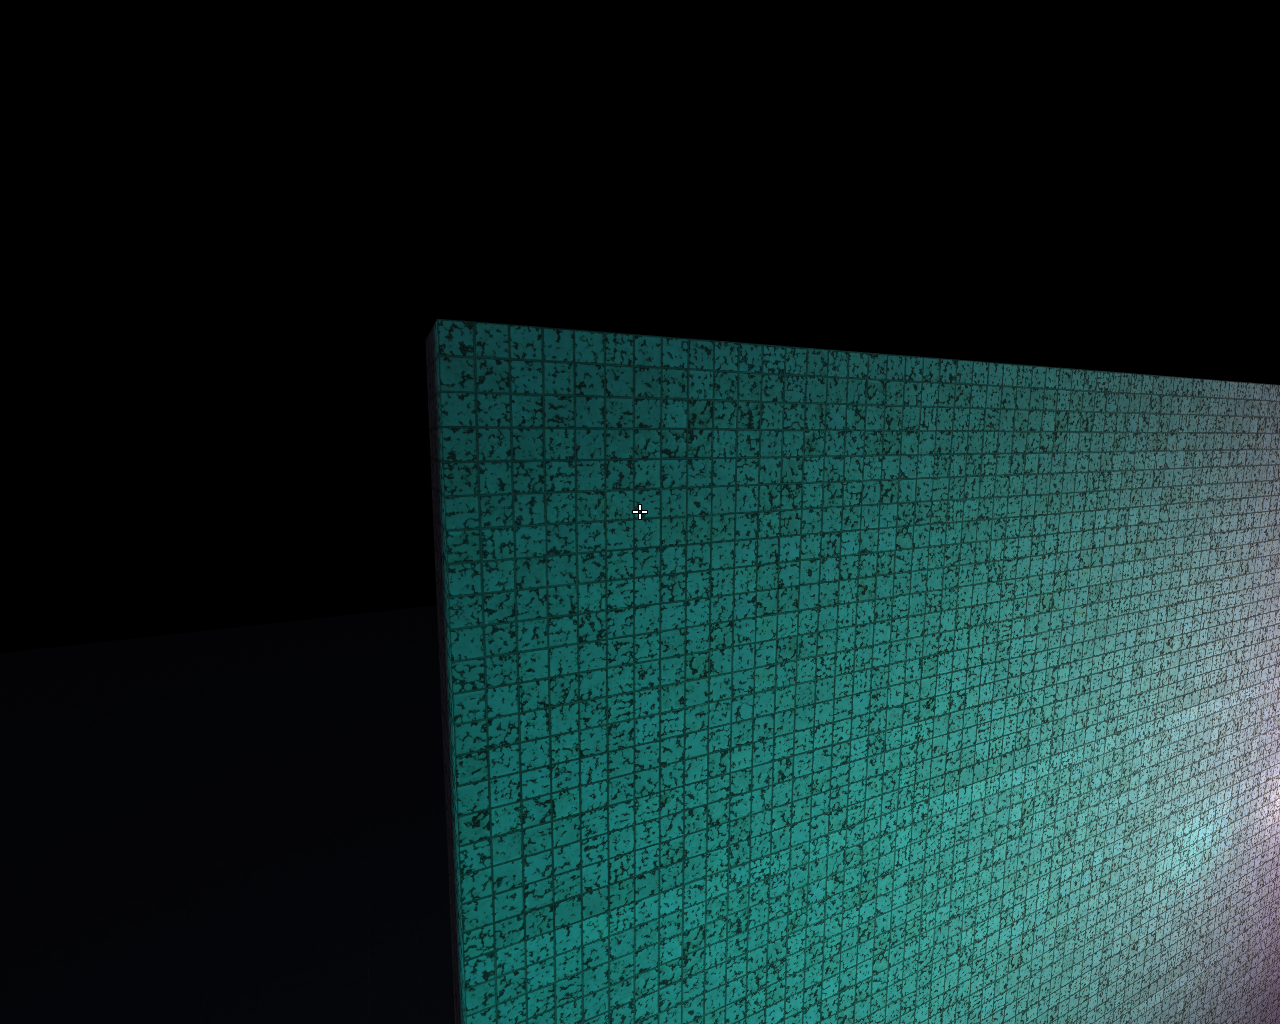
\includegraphics[height=10cm]{images/texture_example.png}
    \caption{Ukázka textury zdi}
    \label{fig:Ukázka textury zdi}
\end{figure}

Na Obrázku \ref{fig:Ukázka textury zdi} vidíme kvádr, který má texturu dlaždiček. Na první pohled tak působí, že se skutečně skládá z několika stovek kostiček, ve skutečnosti se jedná jen o obrázek, dodávající tento dojem. Při tvorbě scény musíme zvážit, jaký pocit má dávat uživateli. Jaký materiál by byl pro těleso vhodný? Jak detailní by samotná textura měla být? Při volbě textury je nutné zvolit takovou texturu, která nebude nevyčnívat a bude dostatečně realistická.

\subsubsection{Světlo} \label{light}

Světlo je nejdůležitějším konceptem, který stojí za vizuální reprezentací čehokoliv, co může člověk vnímat. Ve skutečnosti nevidíme samotná tělesa, nýbrž paprsky světla, které se od těles odráží. Paprsky se mohou dále odrážet, být pohlceny nebo projít tělesem. Simulovat tento proces je ale výkonově vysoce náročné, a přestože s moderními grafickými čipy to možné je, pro naše účely práce nám bude stačit jednodušší řešení. Samotné světlo může mít několik druhů; ty nyní přiblížím. \cite{light}

\vspace{0.5cm}
\begin{figure}[h]
    \centering
    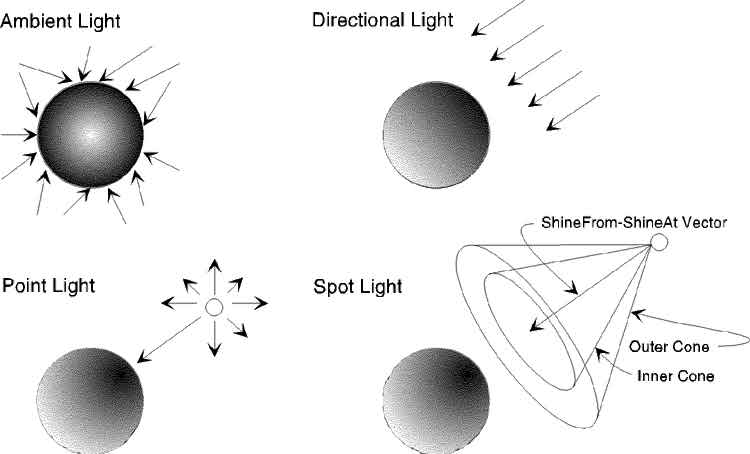
\includegraphics[height=6cm]{images/light_img.jpeg}
    \caption[Různé druhy světel]{Různé druhy světel \cite{light_img}}
    \label{fig:Různé druhy světel}
\end{figure}

Prvním druhem světla je takzvané ambientní světlo — světlo prostředí. Kdybychom večer zhasnuli v místnosti světlo, stále matně uvidíme siluety objektů, potažmo jejich barvy. Důvodem je již zmíněné odrážení světla. Kolem nás je velké množství světelných zdrojů a tedy i nějaká úroveň světla. Na Obrázku \ref{fig:Různé druhy světel} vlevo nahoře vidíme, jak takový druh světla vypadá v praxi. Pokud chceme mít takovéto světlo v programu, musíme nalézt řešení, které není výkonnostně náročné a bude dostačující pro naše účely.

Dalším typem je světlo směrové, které na Obrázku \ref{fig:Různé druhy světel} vidíme vpravo nahoře. Je to světlo, jehož paprsky jsou rovnoběžné; směřují tedy vždy stejným směrem. V praxi se může jednat o slunečný svit, který v malém měřítku (např. oblast města Praha) působí, že svítí na všech místech stejným směrem. Ve velkém měřítku (např. ve sluneční soustavě) už hvězda působí jako jiný typ světla — jde o světlo bodové.

Bodové světlo vidíme na Obrázku \ref{fig:Různé druhy světel} vlevo dole. Je to jeden bod, který všemi směry vyzařuje stejnou sílu světla do prostoru. V praxi to může být žárovka, plamen svíce či hvězda ve vesmíru. Toto světlo se také společně s uplynutou délkou paprsků postupně vytrácí. Tomuto jevu říkáme atenuace světla \cite{attenuation}. Tento děj lze matematicky popsat:

\[f_a = \frac{1}{k_c + d \cdot k_l + d^2 \cdot k_q}\]

Kde $f_a$ popisuje násobek světla v daném bodě, $k_c$ je pak konstantní člen atenuace, $k_l$ lineární člen atenuace, $k_q$ kvadratický člen atenuace a samotné $d$ pak vzdálenost bodu od světelného zdroje. Úpravou těchto parametrů při implementaci můžeme dosáhnout různého chování úpadku světla.

Posledním typem světla jenž popíši je světlo kuželové. Ukázku tohoto světla můžeme vidět na Obrázku \ref{fig:Různé druhy světel}. Laicky by se dalo říci, že se jedná o kombinaci bodového a směrového světla. Jde  o světlo, které svítí z jednoho bodu v definovaném kuželu a stejně jako u bodového světla se jeho síla postupně vytrácí (efekt atenuace). \cite{spotlight}

\subsubsection{GUI}

GUI, jak již zaznělo Graphical User Interface, je druhem uživatelského rozhraní. Umožňuje nám interagovat s programem díky různým symbolům, tlačítkům či ikonám. Rovněž ale může zpětně díky GUI interagovat program s námi. \cite{gui2}

\vspace{0.5cm}
\begin{figure}[h]
    \centering
    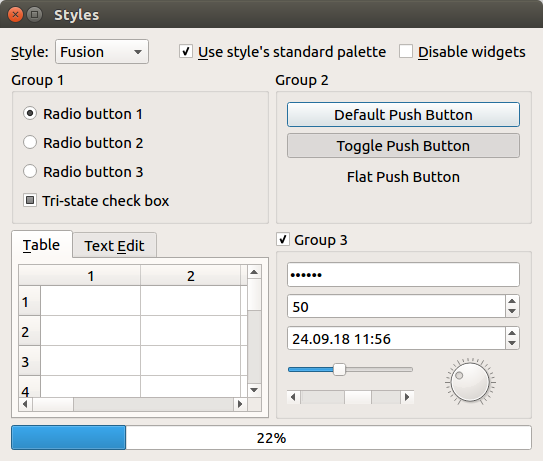
\includegraphics[height=9cm]{images/gui.png}
    \caption[Ukázka různých prvků GUI]{Ukázka různých prvků GUI \cite{gui_img}}
    \label{fig:Ukázka různých prvků GUI}
\end{figure}

Je důležité volit ikony a vzhledy prvků grafického rozhraní tak, abychom mohli snadno odvodit jejich význam a k čemu slouží. Na obrázku \ref{fig:Ukázka různých prvků GUI} vidíme příklad okna, které obsahuje různá tlačítka, tabulku, posuvníky či výběrová pole. Všechny tyto zmíněné prvky jsou určeny pro komunikaci uživatele s programem, nikoliv naopak.

Jak tedy může komunikovat program s uživatelem skrze GUI? Tuto interakci často vidíme ve hrách. Ukazatel počtu životů hráče, náhled mapy herního světa nebo například tachometr vozidla na obrazovce. Nyní popíši implementaci GUI na příkladu.

\vspace{0.5cm}
\begin{figure}[h]
    \centering
    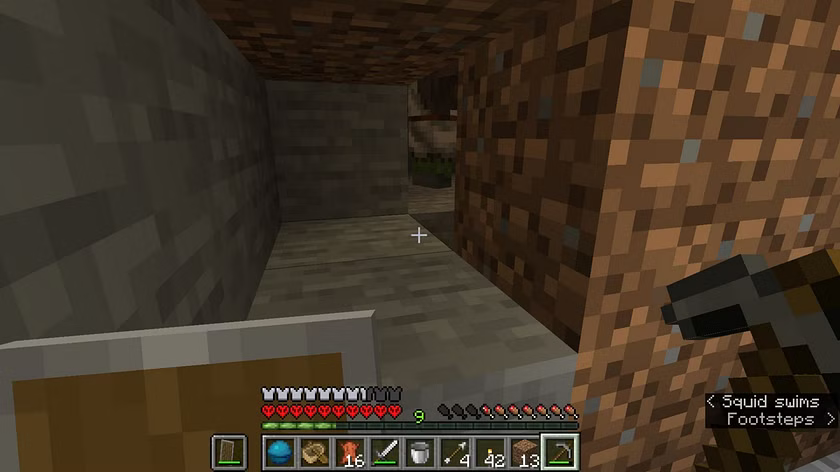
\includegraphics[height=7cm]{images/minecraft.png}
    \caption[Snímek obrazovky ze hry Minecraft]{Snímek obrazovky ze hry Minecraft \cite{minecraft_img}}
    \label{Snímek obrazovky ze hry Minecraft}
\end{figure}

V dolní části Obrázku \ref{Snímek obrazovky ze hry Minecraft} vidíme lištu, společně s několika ikonami. Rudá srdce vlevo ukazují, kolik má hráč bodů života, malé ikonky kusů masa vpravo pak představují, jak moc je hráč nasycený. Ikony železného brnění nad životy popisují, jak kvalitní má hráč výzbroj. Mimo jiné v liště vidíme i některé předměty, která hráč vlastní. Malým detailem jsou i titulky vpravo, které vypisují zvukové události ve hře ze které směru samotný zvuk pochází.

 Takto může hra jednoduše sdělit uživateli informace o jeho stavu a okolí. Není tak potřeba vypisovat text uživateli o tom, zda se jeho postava musí najíst; tato informace je hráči zřejmá díky jednoduchým ikonám. Volba jednoduchý grafických prvků znamená i jejich jednoduché pochopení.

\subsection{Matematické koncepty}

Při tvorbě programu, který pracuje s prostorem, potřebujeme definovat samotný prostor a operace s ním popsat tak, aby jim program rozuměl. Touto problematikou se zabývá lineární algebra. Lineární algebra je odvětví matematiky, které rozvíjí algebru samotnou. Umožňuje nám práci s takzvanými vektory a vektorovým prostorem. lineárními transformacemi a soustavami lineárních rovnic. \cite{linear_algebra} Nyní popíši hlavní komponenty lineární algebry, které je pro správnou implementaci programu nutné pochopit.

\subsubsection{Vektor} \label{vector}

Vektor představuje veličinu, jenž má směr a velikost. Vektor si můžeme představit jako šipku o dané délce (velikosti) s konkrétním směrem. Jedná se o soubor seřazených hodnot. Vektory zapisujeme malými písmeny se šipkou nad písmenem ($\vec{a}$). Také je lze zapsat jako názvy bodů bez mezer s šipkou nad ($\vec{AB}$). \cite{vector}

Nyní budou popsány základní operace s vektory. Vektory můžeme např. sčítat, odečítat, získat jejich velikost, násobit číslem nebo získat tzv. skalární a vektorový součin, jenž popíšu na konci kapitoly. Sčítání vektorů je komutativní operace (nezáleží nám na jejich pořadí). Součtem vektorů vzniká vektor další, kde každá jeho složka je součtem složek vektorů sčítaných.

Vektory $\vec{a}$ a $\vec{b}$ jsou zapsány jako:
\begin{align}
    \vec{a} &= (4, -1, 2), \notag \\
    \vec{b} &= (-3, 8, -3).
\end{align}

Jejich součet $\vec{c} = \vec{a} + \vec{b}$ je pak:
\begin{align}
    \vec{c} &= (4 + (-3), (-1) + 8, 2 + (-3)) \notag \\
      &= (1, 7, -1).
\end{align}

\pagebreak

Stejným způsobem pak můžeme vektory odečítat; stačí záměna znaménka plus za znaménko minus. Odčítání vektorů je velmi užitečné, neboť máme-li body A a B s různými souřadnicemi, odečtem jejich souřadnic vyjádřených vektory získáváme tzv. vektor směrový. Směrový vektor popisuje směr mezi těmito body. V praxi tak můžeme popsat např. směr pohledu kamery — odečtem pozice kamery od bodu, na který cílí.

Považujme pozici kamery za bod $A$ a cílový bod za bod $B$, pak směrový vektor $\vec{AB}$ vypočteme takto:
\begin{align}
    \vec{AB} &= B - A
\end{align}

\vspace{0.5cm}
\begin{figure}[h]
    \centering
    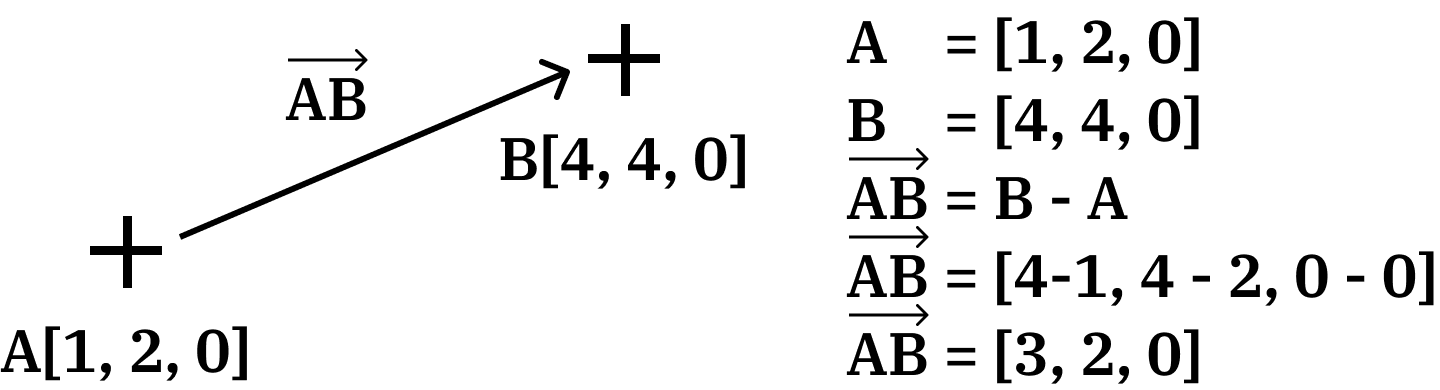
\includegraphics[height=2.5cm]{images/vector_sub.png}
    \caption{Směrový vektor $\vec{AB}$}
    \label{fig:Směrový vektor AB}
\end{figure}

Na Obrázku \ref{fig:Směrový vektor AB} vidíme zakreslené naše body $A$ a $B$. Šipka mezi těmito body představuje směrový vektor $\vec{AB}$. Následně od sebe odečítáme jejich jednotlivé složky a získáváme hodnotu směrového vektoru. Další podstatnou operací při práci s vektory je získání jejich velikosti. Tento proces vychází z Pythagorovy věty \cite{pythagorean_theorem}. Mějme vektor $\vec{a}$:
\begin{align}
    \vec{a} &= (4, 3)
\end{align}

Pak je velikost tohoto vektoru rovna:
\begin{equation}
    |\vec{a}| = \sqrt{4^2 + 3^2} = \sqrt{25} = 5
\end{equation}

Obecně lze pak tvrdit, že velikost vektoru je rovna druhé odmocnině součtu druhých mocnin jeho složek. Vzorec pro získání velikosti n-dimenzionálního vektoru $\vec{v}$ vypadá následovně:
\begin{equation}
    |\vec{v}| = \sqrt{\sum_{i = 1}^{n} (\vec{v}_i)^2}
\end{equation}

V tomto vzorci představuje $n$ počet dimenzí (složek) vektoru, kde $n \in \mathbb{N}$. Chceme-li využít vektor pro reprezentaci směru v prostoru, jeho délka nás pravděpodobně nezajímá. Ideální by bylo mít vektor, který má délku rovnou právě 1. Když známe velikost vektoru, můžeme velikost upravit tak, aby měl velikost 1 a jeho směr zůstal zachován. Tomuto procesu říkáme normalizace vektoru, jehož výsledkem je vektor jednotkový (normalizovaný). Takovýto vektor značíme stříškou (vokání) nad jeho názvem. Stačí nám pouze vydělit jednotlivé složky vektoru jeho délkou:
\begin{equation}
    \hat{v} = \frac{\vec{v}}{|\vec{v}|} = \frac{\vec{v}}{\sqrt{\sum_{i = 1}^{n} (\vec{v}_i)^2}}
\end{equation}

Pro ukázku uvedu vektor $\vec{a}$ a získání jeho jednotkové verze ($\hat{a}$):
\begin{align}
    \vec{a} &= (5, 12, 0) \notag \\
    |\vec{a}| = \sqrt{5^2 + 12^2 + 0^2} &= \sqrt{25 + 144 + 0} = \sqrt{169} = 13 \notag \\
    \hat{a} = \frac{(5, 12, 0)}{13} &= (\frac{5}{13}, \frac{12}{13}, 0)
\end{align}

Další operace, která bude představena je tzv. skalární součin. Skalární součin dvou vektorů nám říká, jak podobné jsou směry, jímž vektory ukazují. Výsledkem této operace je jedna číselná hodnota Získáme ji součtem součinu první složky vektoru $\vec{a}$ a vektoru $\vec{b}$, následně součinu složek druhých, dokud nevyčerpáme všechny složky. V případě, že je skalární součin dvou nenulových vektorů roven číslu 0, pak jsou tyto vektory na sebe kolmé. Skalární součin zapisujeme jako standardní násobení (např. $\vec{a} \cdot \vec{b}$).

Takto vypadá výpočet skalárního součinu pro vektory $\vec{a}$ a $\vec{b}$:
\begin{align}
    \vec{a} &= (-4, -1, 2), \notag \\
    \vec{b} &= (-3, 8, 3) \notag \\
    \vec{a} \cdot \vec{b} &= (-4) \cdot (-3) + (-1) \cdot 8 + 2 \cdot 3 \notag \\
    \vec{a} \cdot \vec{b} &= 12 + (-8) + 6 = 10
\end{align}

Tento proces můžeme zobecnit tímto vzorcem:
\begin{equation}
    \vec{a} \cdot \vec{b} = \sum_{i=1}^{n}(\vec{a}_i \cdot \vec{b}_i)
\end{equation}

V tomto vzorci opět $n$ představuje počet dimenzí vektoru, přičemž platí $n \in \mathbb{N}$. Nyní detailněji představím operaci, která se nazývá vektorový součin. Vektorový součin je standardně definován pouze pro třídimenzionální vektory. Výsledkem vektorového součinu dvou vektorů $\vec{a}$ a $\vec{b}$ (zapíšeme $\vec{a} \times \vec{b}$) je vektor, jenž je kolmý na $\vec{a}$~i~$\vec{b}$.

\vspace{0.5cm}
\begin{figure}[h]
    \centering
    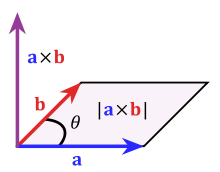
\includegraphics[height=3cm]{images/cross_product.png}
    \caption[Vektorový součin dvou vektorů]{Vektorový součin dvou vektorů \cite{gui_img}}
    \label{fig:Vektorový součin dvou vektorů}
\end{figure}

Pro $\vec{a}$ a $\vec{b}$ platí, že:
\begin{equation}
    \vec{a} \times \vec{b} = \begin{pmatrix}
        a_2 \cdot b_3 - a_3 \cdot b_2, \\
        a_3 \cdot b_1 - a_1 \cdot b_3, \\
        a_1 \cdot b_2 - a_2 \cdot b_1
    \end{pmatrix}
\end{equation}

Pro lepší představu o výpočtu demonstruji vektorový součin na příkladu:
\begin{align}
    \vec{a} &= (3, 4, -1), \notag \\
    \vec{b} &= (1, 7, -9)
\end{align}
\begin{equation}
    \vec{a} \times \vec{b} = \begin{pmatrix}
        4 \cdot (-9) - (-1) \cdot 7, \\
        (-1) \cdot 1 - 3 \cdot (-9), \\
        3 \cdot 7 - 4 \cdot 1
    \end{pmatrix} = \begin{pmatrix}
        -29 \\
        26, \\
        17 \cdot 7 - 4 \cdot 1
    \end{pmatrix}
\end{equation}

Nakonec uvedu, že vektory lze násobit (a tedy i dělit) jedním číslem. Toto číslo se nazývá skalár a bývá označováno řeckým písmenem lambda — $\lambda$. Tato operace pro třírozměrný vektor vypadá následovně:
\begin{equation}
    \lambda \cdot \vec{v} = (\lambda \cdot \vec{v}_1, \lambda \cdot \vec{v}_2, \lambda \cdot \vec{v}_3)
\end{equation}

Zde vidíme i příklad s konkrétními hodnotami:
\begin{equation}
    3 \cdot (4, 7, 3) = (3 \cdot 4, 3 \cdot 7, 3 \cdot 3) = (12, 21, 9)
\end{equation}

\subsubsection{Matice}

Matice je souborem hodnot, který můžeme rozdělit na sloupce a řádky. Jednotlivé hodnoty v ní nazýváme prvky množiny. U matic můžeme určit jejich rozměr (řád), který je udávaný jako počet řádků krát počet sloupců (např. $2 \times 3$). Tento řád můžeme u matice zapsat dolním indexem. \cite{matrix}

Zde je příklad matice $A$ s různými hodnotami, která má právě tři řádky a tři sloupce:
\begin{equation}
    A = \begin{bmatrix}
        1 & 2 & 3 \\
        4 & 5 & 9 \\
        7 & 8 & 10
    \end{bmatrix}_{3 \times 3}
\end{equation}

Tato konkrétní matice je zároveň příkladem speciálního druhu matic, neboť má stejný počet řádků a sloupců — jedná se o matici čtvercovou. Matice lze využívat více způsoby, pro práci je relevantní využití při transformacích (přeměnách) prostoru. Může se jednat o rotaci, posun či např. zkosení. Pro matice je stejně jako u vektorů definováno několik operací. Začnu popisem sčítání dvou matic.

Chci-li sčítat matice $A$ a $B$, pak musí býti jejich rozměry stejné. Pokud je tato podmínka splněna, mohu sčítat jednotlivé prvky tak, že do nové matice vložím součet prvků na dané pozici matic $A$ a $B$. Pro 2 matice o řádu $3 \times 3$:
\begin{equation}
    A + B = \begin{bmatrix}
        a_{11} + b_{11} & a_{12} + b_{12} & a_{13} + b_{13} \\
        a_{21} + b_{21} & a_{22} + b_{22} & a_{23} + b_{23} \\
        a_{31} + b_{31} & a_{32} + b_{32} & a_{33} + b_{33}
    \end{bmatrix}_{3 \times 3}
\end{equation}

Malé písmeno nám říká, že se jedná o prvek dané matice, dolní index pak prvním číslem udává řádek prvku a druhým číslem jeho sloupec. Např. $a_{23}$ je prvek matice $A$, jenž se nachází v druhém řádku a třetím sloupci. Nyní následuje ukázka, jak toto sčítání vypadá v praxi:
\begin{align}
    \begin{bmatrix}
        3 & 9 & -2 \\
        2 & -4 & -9 \\
        8 & 3 & 0
    \end{bmatrix} + \begin{bmatrix}
        9 & -1 & 5 \\
        -3 & 0 & -1 \\
        1 & 5 & 10
    \end{bmatrix} &= \begin{bmatrix}
        3 + 9 & 9 + (-1) & (-2) + 5 \\
        2 + (-3) & (-4) + 0 & (-9) + (-1) \\
        8 + 1 & 3 + 5 & 0 + 10
    \end{bmatrix} \notag \\
    &= \begin{bmatrix}
        12 & 8 & 3 \\
        -1 & -4 & -10 \\
        9 & 8 & 10
    \end{bmatrix}
\end{align}

Rozdíl dvou matic ($A - B$) je pak identický, stejně jako u vektorů nám postačí změna znaménka plus na minus. Součet a rozdíl nejsou jediné operace, které mají matice a vektory společné. Matice můžeme násobit skalárem (číslem) tak, že každý prvek budeme touto hodnotou násobit. V případě násobení matice $A$ řádu $3 \times 3$ skalárem $\lambda$, lze tuto operaci zobecnit takto:
\begin{equation}
    \lambda \cdot A = \begin{bmatrix}
        \lambda \cdot a_{11} & \lambda \cdot a_{12} & \lambda \cdot a_{13} \\
        \lambda \cdot a_{21} & \lambda \cdot a_{22} & \lambda \cdot a_{23} \\
        \lambda \cdot a_{31} & \lambda \cdot a_{32} & \lambda \cdot a_{33}
    \end{bmatrix}_{3x3}
\end{equation}

Kdybychom dosadili za $\lambda$ např. číslo $4$ a zvolili hodnoty pro matici, pak by dosazení vypadalo takto:
\begin{equation}
    4 \cdot \begin{bmatrix}
        3 & 9 & -2 \\
        2 & -4 & -9 \\
        8 & 3 & 0
    \end{bmatrix} = \begin{bmatrix}
        4 \cdot 3 & 4 \cdot 9 & 4 \cdot  (-2) \\
        4 \cdot 2 & 4 \cdot (-4) & 4 \cdot (-9) \\
        4 \cdot 8 & 4 \cdot 3 & 4 \cdot 0
    \end{bmatrix} = \begin{bmatrix}
        12 & 36 & -8 \\
        8 & -16 & -36 \\
        32 & 12 & 0
    \end{bmatrix}
\end{equation}

Všechny předešlé operace pro práci s maticemi byly vcelku intuitivní. Větší problém je násobení matice maticí. Aby bylo možné vynásobit matici $A$ maticí $B$, musí být splněna podmínka, že má matice $A$ stejný počet sloupců, jako má matice $B$ řádků. Následně se provádí skalární součin vektorů řádkových první matice s vektory sloupcovými matice druhé. Matematicky zapíšeme jako:
\begin{equation}
    (A \cdot B)_{ij} = \sum_{p=1}^{n}(a_{ip} \cdot {b_{pj}})
\end{equation}
\begin{figure}[h]
    \centering
    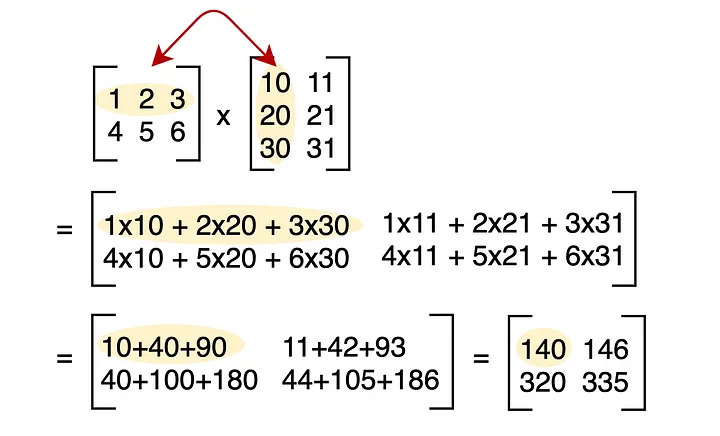
\includegraphics[height=4.2cm]{images/matrix_mp.png}
    \caption[Vizualizace násobení matic]{Vizualizace násobení matic \cite{matrix_mp_img}}
    \label{fig:Vizualizace násobení matic}
\end{figure}
\section{Implementace}

V této kapitole se zabývám implementací konceptů, které jsem vysvětlil v kapitole předešlé. Vypíši, jaké externí knihovny jsou využity pro jaké funkce, na jakém principu fungují jednotlivé části kódu a popíši, jak probíhal jejich vývoj. V sekci také budou ukázky kódu vysvětlovaných částí.
\subsection{Externí knihovny}

Engine využívá několik externích knihoven pro své fungování. Pro připomenutí, knihovna je již hotový kód, který řeší daný problém. Důvodem je praktičnost, neboť tvorba enginu bez jakýkoliv dalších knihoven, který bude podporován více platformami naráz, by byla velmi zdlouhavá. Kvalitně řešit některé problémy by znamenalo mít rozsáhlé zkušenosti s OpenGL, jeho implementačními detaily, správou oken na různých operačních systémech či s různými datovými formáty. Snažím se o nejmenší počet externích knihoven, abych mohl mít co nejvíce vlastních, ovlivnitelných částí; v projektu jsou takovéto knihovny tři:

\begin{enumerate}
    \item GLFW \cite{glfw} — knihovna pro multiplatformní tvorbu a správu okna.
    \item GLEW \cite{glew} — knihovna pro načtení OpenGL funkcí.
    \item libPNG \cite{libpng} — knihovna pro načítání obrázků ve formátu PNG.
\end{enumerate}

Jedná se o velmi rozšířené knihovny, které se při tvorbě enginů v jazyce C++ často využívají. GLFW podporuje i další grafická rozhraní mimo OpenGL, např. Vulkan či OpenGL ES, o kterých jsem již mluvil v kapitole \ref{g_interface}. Nejen že podporuje více grafických rozhraní, podporuje i více operačních systémů a display serverů. GLEW nám řekne, kde najít jakou OpenGL funkci a díky němu jich tak můžeme využívat. Také je schopné detekovat schopnosti platformy, na které engine spouštíme. Můžeme tak dynamicky optimalizovat či upravit logiku dle zařízení uživatele.

Knihovna libPNG, jak z názvu vyplývá, řeší čtení a zápis ve formátu PNG. PNG je zkratka pro Portable Network Graphics pro ukládání rastrových obrázků. Tento formát podporuje různé velikosti barevných palet (ta ovlivňuje, kolik může obrázek používat barev naráz), kompresi dat, pro úspornější využití místa disku či průhlednost. Knihovna je pro příklad schopna obrázek načíst jako skupinu bytů, zjistit jeho rozměry (výšku a šířku), zda obrázek využívá průhlednost nebo zjistit jeho barevnou paletu. Samotná historie knihovny libPNG sahá až do roku 1995.

\subsection{Build systém}

C++ musíme zkompilovat (převést) do spustitelného kódu. Tohoto docílíme jiným programem — compilerem. Úkolem compileru je právě převádění zdrojového kódu (který píše programátor) na kód zdrojový (pro počítač). Mezi rozšířené compilery pro tento jazyk patří g++ \cite{gnu_gcc}, LLVM \cite{llvm} či MSVC \cite{msvc}. Compiler není závislý na implementaci, není tedy pro práci nutné konkrétní compiler volit. Kdybychom chtěli spouštět kód, museli bychom se dobře naučit s compilerem, říct mu, kde najde jakou knihovnu, soubory a s jakými nastaveními má kód budovat. Automatizování tohoto procesu by bez speciální logiky fungovalo pouze pro danou platformu. Řešením je využívání build systému — systému určený pro budování aplikací.

Jeden z nástrojů automatizace jsou takzvané Makefiles \cite{makefile}. Jedná se o soubory, které generalizují kompilační proces a projekt se nám pak dle těchto požadavků zpracuje. Prakticky nám tak stačí využívat Makefiles pro budování projektu s podporou více compilerů. Build systémy nám umožňují jednodušší práci s Makefiles a jejich snadnou správu. Příkladem je build systém CMake \cite{cmake}, který používá své vlastní soubory pro tvorbu Makefiles. Tento systém je využit mou prací, neboť je velmi rozšířen a podporován. Také mohu lépe řešit logiku detekce operačního systému uživatele při tvorbě programu, než kdybych používal Makefiles samotné.

\vspace{0.5cm}
\begin{figure}[h]
    \centering
    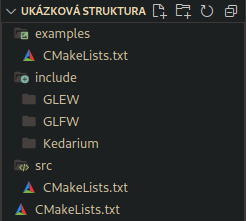
\includegraphics[height=3.5cm]{images/fs.png}
    \caption{Ukázka CMake souborů v projektu}
    \label{fig:Ukázka CMake souborů v projektu}
\end{figure}

\pagebreak

Na Obrázku \ref{fig:Ukázka CMake souborů v projektu} vidíme, jak jsou v projektu soubory pro CMake rozloženy. Tyto soubory se vždy jmenují "CMakeLists.txt". Jeden tento soubor je přímo v kořenovém adresáři projektu. Ten odkazuje na CMake soubory v jednotlivých složkách projektu. Jedná se o soubor ve složce \mintinline{bash}{/src}, kde se nachází zdrojový kód knihovny. Podobný je soubor ve složce \mintinline{bash}{/examples}, kde jsou ukázkové příklady knihovny. Důležitá je i složka \mintinline{bash}{/include}, kde se nacházejí externí knihovny a knihovna enginu. Po spuštění CMake vytvářím složku \mintinline{bash}{/build}, kde se nachází vygenerovaný Makefile. Z něho se následně tvoří spustitelná aplikace, pro ukázku:

\vspace{0.5cm}
\begin{figure}[h]
    \centering
    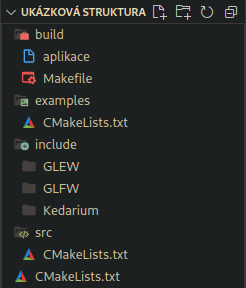
\includegraphics[height=5.5cm]{images/fs_2.png}
    \caption{Ukázka CMake souborů v projektu po buildu}
    \label{fig:Ukázka CMake souborů v projektu po buildu}
\end{figure}

\subsection{Okno}

Pro logiku okna jsem vytvořil vlastní třídu, ze které si následně uživatel tvoří třídu děděnou. Tato třída obsahuje parametry jako titulek, šířku, výšku, GLFW instanci okna či odkaz na jeho aktivní kameru. Pro parametry třídy jsou definovány i gettery a settery pro jejich úpravy či získání. Některé metody jsou přímo určeny pro implementaci potomky třídy. Jedná se například o metody \mintinline{cpp}{update} a \mintinline{cpp}{render}.

Tato třída také spravuje takzvaný delta time — čas uplynutý mezi snímky \cite{delta_time}. Představme si, že na obrazovce nám běhá postavička. Ta by měla běžet rychlostí $10$. Každý snímek tak ujde právě 10 pixelů. Co když mám ale pomalé zařízení či monitor s vyšší zobrazovací frekvencí? Výsledky se pak mohou několiknásobně lišit. Při násobení rychlost $10$ hodnotou delta time tento rozdíl odstraňujeme.

\vspace{0.5cm}
\begin{figure}[h]
    \centering
    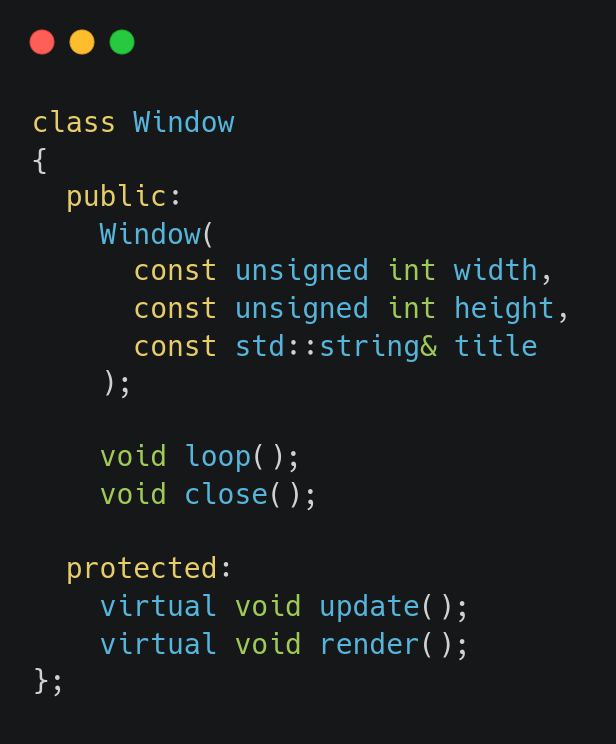
\includegraphics[height=7cm]{images/window_code.png}
    \caption{Zjednodušený kód třídy Window}
    \label{fig:Zjednodušený kód třídy Window}
\end{figure}

Na Obrázku \ref{fig:Zjednodušený kód třídy Window} vidíme zjednodušený kód pro tuto třídu. Tento obrázek jsem tvořil pomocí online nástroje Carbon pro tvorbu obrázků kódu \cite{carbon}. Třída však obsahuje i další logiku, kupříkladu pro maximalizaci a minimalizaci okna. Jak vidíme, okno má zmíněné metody \mintinline{cpp}{update} a \mintinline{cpp}{render}, dále pak metodu \mintinline{cpp}{loop}, která spustí hlavní cyklus (střídání aktualizace a vykreslování) a metodu \mintinline{cpp}{close} pro zavření okna. Potom této třídy by mohl vypadat následovně:

\vspace{0.5cm}
\begin{figure}[h]
    \centering
    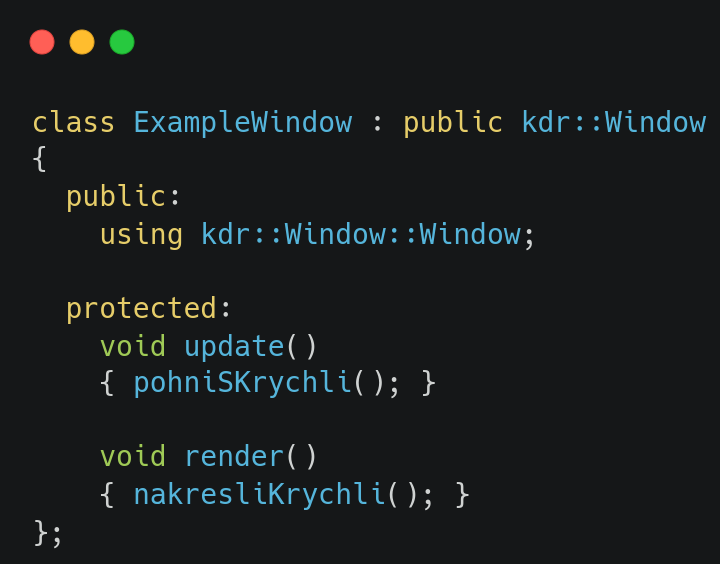
\includegraphics[height=5.5cm]{images/window_child_code.png}
    \caption{Zjednodušená dědičná třída z Window}
    \label{fig:Zjednodušená dědičná třída z Window}
\end{figure}

\pagebreak

Jak vidíme na obrázku \ref{fig:Zjednodušená dědičná třída z Window}, třída nevychází přímo z \mintinline{cpp}{Window} ale z \mintinline{cpp}{kdr::Window}. Jednotlivé moduly enginy jsou uvnitř namespace (představme si ho jako balíček) se zkratkou \mintinline{cpp}{kdr} (zkráceně Kedarium). Důvodem jsou kolize pojmenování při integrace do existujícího projektu. Pokud by měl vývojář vlastní třídu pro správu okna, pak by byli v jeho projektu 2 třídy \mintinline{cpp}{Window}. Namespace tyto problémy řeší a tento princip nacházíme ve všech částech enginu.

\subsection{Správa vstupu}

Pro interakci uživatele s programem je nutné od něj získávat vstup. Správu vstupu v okně řeší používaná knihovna GLFW. Pro unsnadnění práce jsem si vytvořil enumeraci pro jednotlivé klávesy, což je množina předem definovaných hodnot. \cite{enum} Dále má engine funkci, která nám říká, zda je zvolená klávesa aktuálně stisknutá. Zde je ukázka této enumerace a funkce:

\vspace{0.5cm}
\begin{figure}[h]
    \centering
    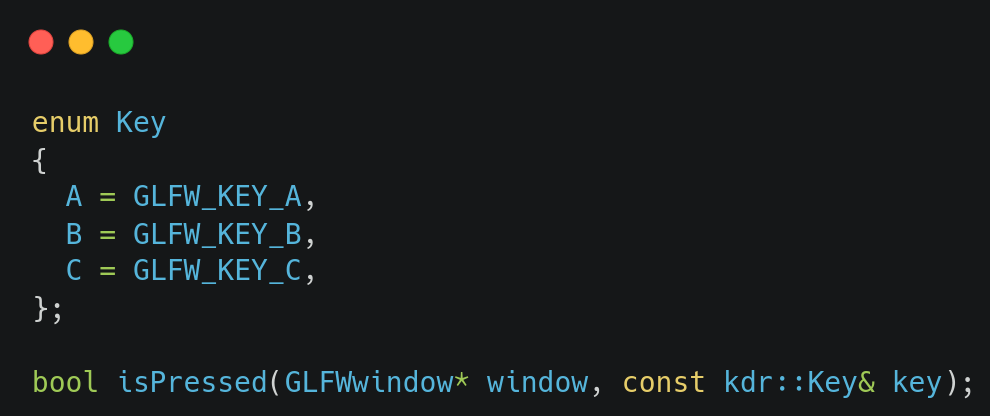
\includegraphics[height=4cm]{images/keys.png}
    \caption{Ukázka enumerace pro klávesy a funkce s ní spojená}
    \label{fig:Ukázka enumerace pro klávesy a funkce s ní spojená}
\end{figure}

Na Obrázku \ref{fig:Ukázka enumerace pro klávesy a funkce s ní spojená} vidíme enumeraci \mintinline{cpp}{Key}, která je využita i ve funkci \mintinline{cpp}{isKeyPressed}. Tato funkce vrací booleovskou hodnotu dle toho, zda je zvolená klávesa v dané GLFW instanci stisknuta. Mohli bychom ji například využít v metodě \mintinline{cpp}{update} ve třídě \mintinline{cpp}{Window} pro rotaci nějakého tělesa. V ukázkových příkladech ji využívám pro změnu módu vykreslování, zvětšení aplikace na celé okno či zamknutí kurzoru myši.

\pagebreak

\subsection{Barvy}

V mé práci abstrahuji barvy do vlastní struktury. Struktura nám seskupuje více informací do jednoho celku. Její součástí ale není chování, čímž se zásadně liší od třídy. \cite{struct} Pro barvu se hodí, neboť barvu lze popsat kombinací několika hodnot. Zde je ukázka, jak vypadá struktura RGBA, která právě tento formát barvy reprezentuje:

\vspace{0.5cm}
\begin{figure}[h]
    \centering
    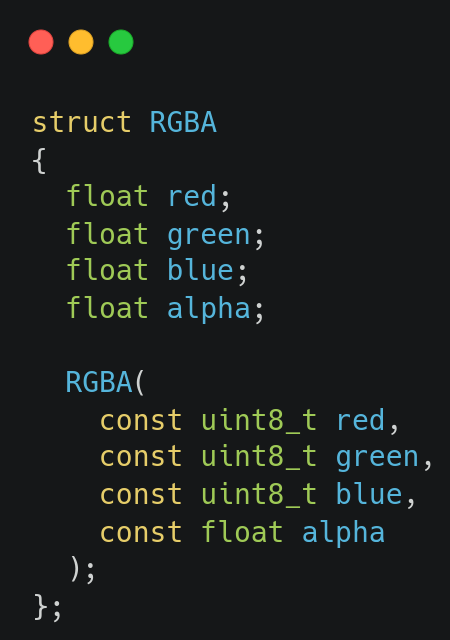
\includegraphics[height=7cm]{images/rgba.png}
    \caption{Struktura RGBA v enginu}
    \label{fig:Struktura RGBA v enginu}
\end{figure}

Tato struktura má 4 hodnoty, jak můžeme vidět na Obrázku \ref{fig:Struktura RGBA v enginu}. Jedná se o sílu barvy červené, zelené a modré, pak o její průhlednost. V konstruktoru mají barvy datový typ \mintinline{cpp}{uint8_t}, který reprezentuje osmi-bitovou hodnotu (0 - 255). Kdybychom zvolili jiný typ, např. \mintinline{cpp}{int}, mohli bychom do konstruktoru vložit i jinou hodnotu, než v tomto rozmezí.

Poslední hodnotou, jak bylo zmíněno, můžeme změnit průhlednost. Tato hodnota je reprezentována datovým typem \mintinline{cpp}{float} a jedná se o desetinné číslo v intervalu $[0; 1]$. Součástí enginu jsou i některé předem definované barvy, abychom nemuseli některé často používané barvy definovat sami. Příkladem může být \mintinline{cpp}{kdr::Color::Black} nebo \mintinline{cpp}{kdr::Color::Red}.

\pagebreak

\subsection{Shadery}

Shadery jsem již zmiňoval v kapitole \ref{opengl}, kde se zabývám OpenGL. Jedná se o malé programy, které mění vstup na výstup v jednotlivých fázích pipeline OpenGL. Pro shader jsem vytvořil vlastní třídu, která shader přečte ze specifikovaných souborů (ty třída dostane jako cesty k nim), spustí nutné OpenGL funkce. Programátorovi dává metody pro aktivaci, mazání a úprav hodnot shaderu. Zde je jeho zjednodušená verze:

\vspace{0.5cm}
\begin{figure}[h]
    \centering
    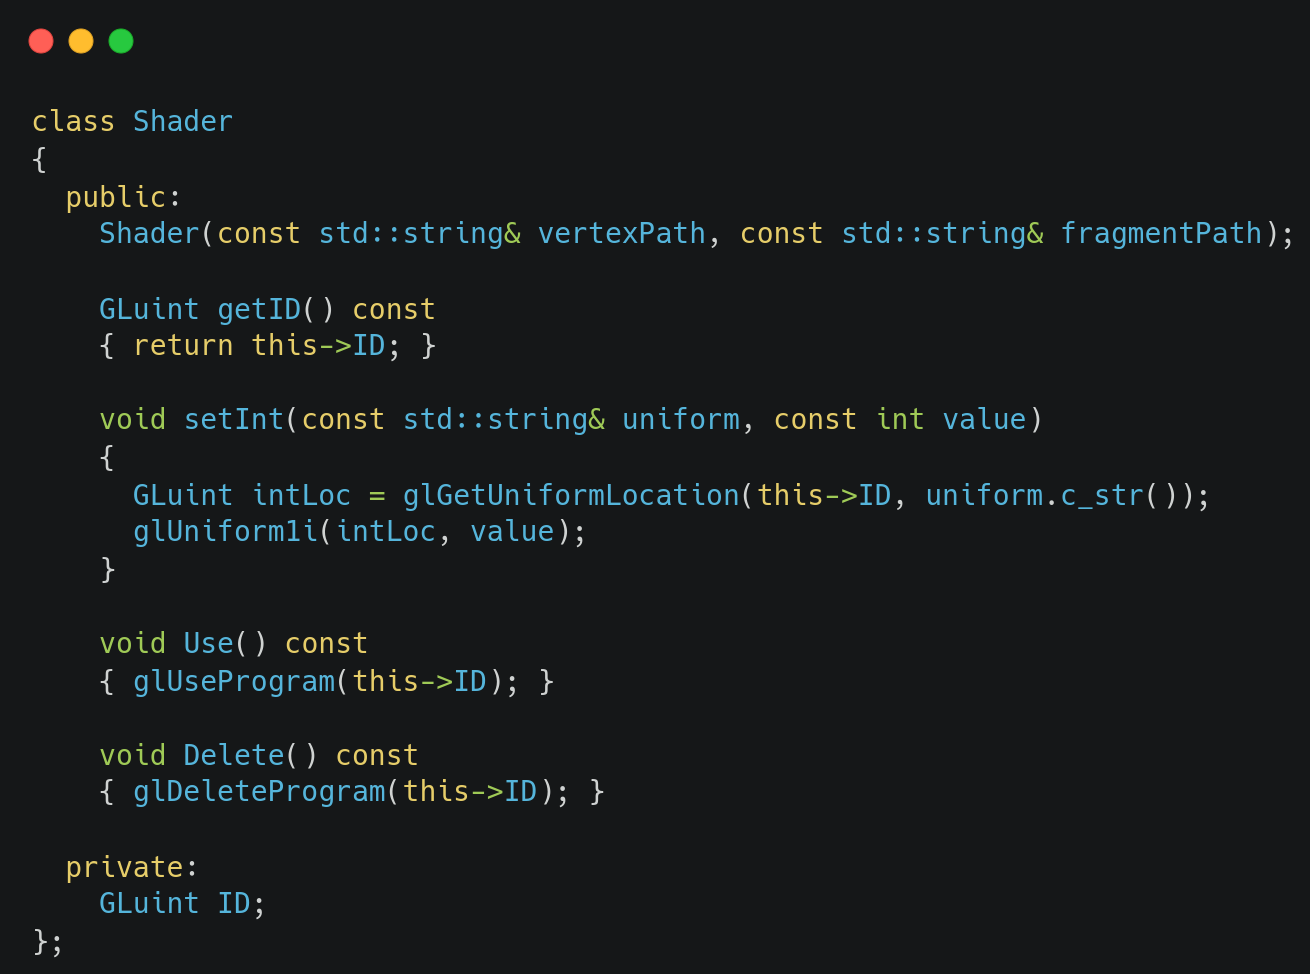
\includegraphics[height=9cm]{images/shader.png}
    \caption{Třída Shader}
    \label{fig:Třída Shader}
\end{figure}

Vidíme zde metody \mintinline{cpp}{Use} a \mintinline{cpp}{Delete}, které shader aktivují a mažou. Na ukázku jsem pro obrázek ponechal metodu \mintinline{cpp}{setInt}, které v shaderu nastaví celočíslenou hodnotu. OpenGL musí vědět, kde danou hodnotu najde a díky metodám pro nastavování hodnot nemusí vývojář využívat OpenGL funkce pro získání jejich lokací. Stačí mu pouze znát, jak hodnotu v souboru s kódem pro shader pojmenoval. Každý shader má také ID, jenž získá při jeho vytvoření.

\pagebreak

\subsection{VAO, VBO a EBO}

VAO, VBO a EBO mají stejně jako shadery vlastní třídy, které práci s nimi usnadňují. Důvodem, proč jsou ve stejné kapitole je, že tyto tři koncepty spolu velmi úzce souvisí a fungují na podobných principech. Stejně jako shader, jedním z jejich parametrů je jejich ID, vygenerované OpenGL při jejich tvorbě. Dále mají tři společné metody, pro jejich aktivaci, deaktivaci a smazání. Pro ukázku začnu uvedením zjednodušeného kódu pro VBO a EBO, které jsou si velmi podobné a liší se pouze v detailech:

\vspace{0.5cm}
\begin{figure}[h]
    \centering
    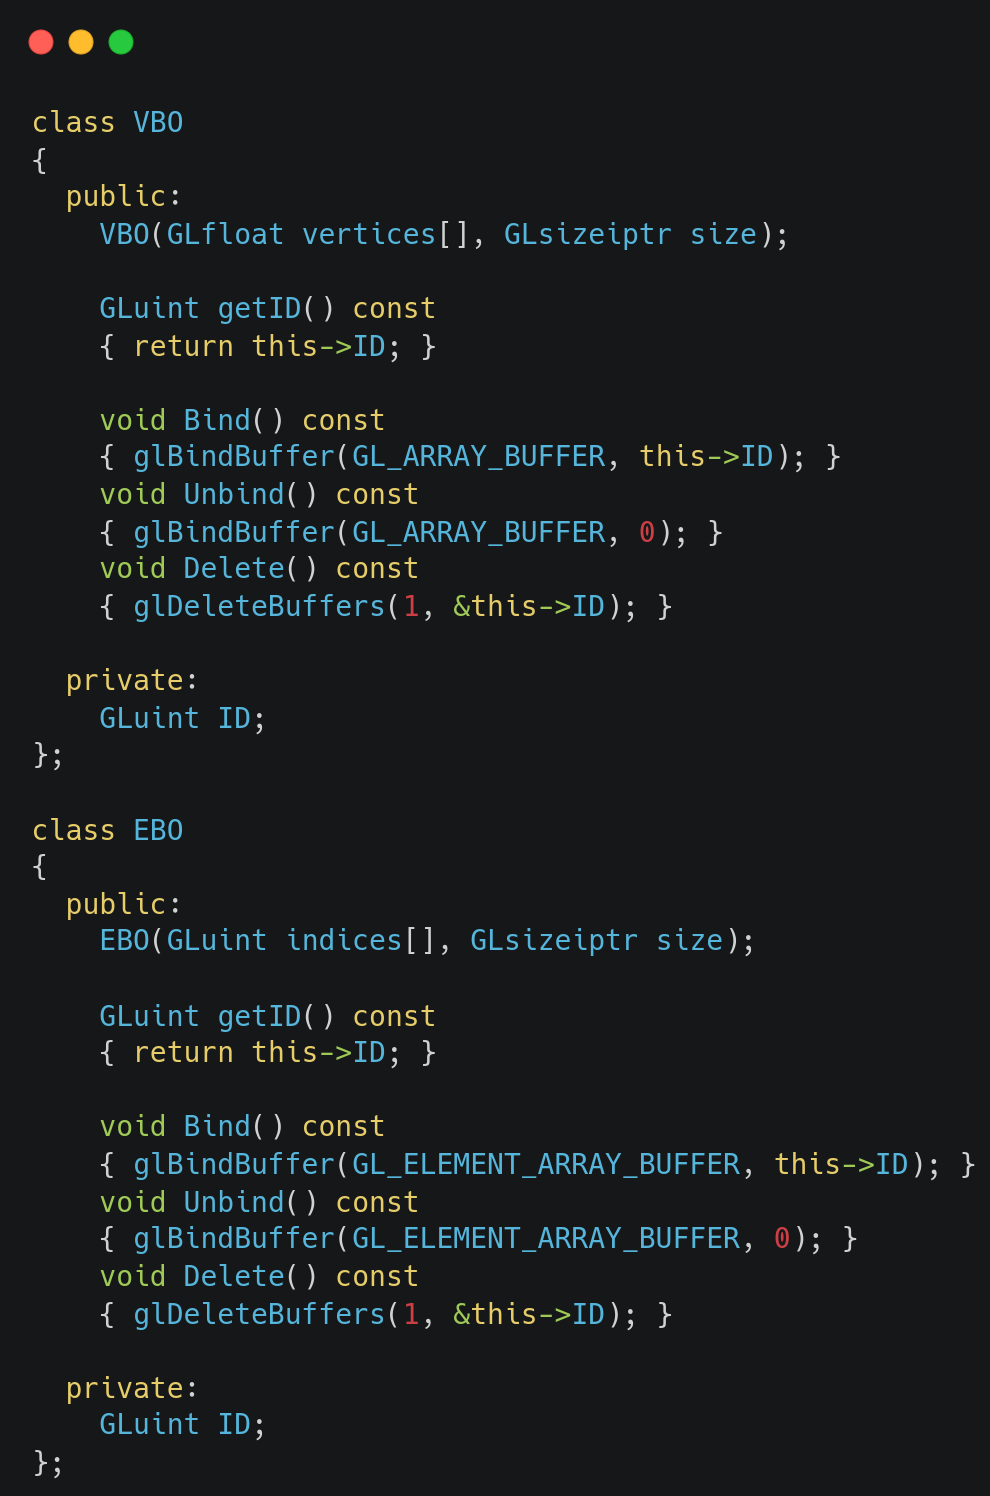
\includegraphics[height=12.5cm]{images/vbo_ebo.png}
    \caption{Třídy VBO a EBO}
    \label{fig:Třídy VBO a EBO}
\end{figure}

\pagebreak

Na Obrázku \ref{fig:Třídy VBO a EBO} vidíme, že se tyto třídy téměř neliší. V úvodu této kapitoly jsem zmiňoval metody pro práci s nimi — jde o metody \mintinline{cpp}{Use}, \mintinline{cpp}{Unbind} a \mintinline{cpp}{Delete}. Při tvorbě VBO musíme do jejího konstruktoru předat pole s daty o vrcholech typu \mintinline{cpp}{GLfloat} (OpenGL typ pro desetinná čísla) a pak velikost tohoto pole. Důvodem předání velikosti pole je, že v programovacích jazycích C a C++ se pole při přidání ve funkci mění na ukazatel na něj. Stejným způsobem pak tvoříme instance EBO, předáváme ale pole s hodnotami typu \mintinline{cpp}{GLuint} (OpenGL typ pro nezáporné celé číslo). Jedná se o instrukce pro vykreslení trojúhelníků.

Třída VAO je podobná, obsahuje ale navíc metodu pro zavedení atributů (např. pozice či barva) a při její tvorbě žádné parametry nepředáváme. Zjednodušená třída vypadá následovně:

\vspace{0.5cm}
\begin{figure}[h]
    \centering
    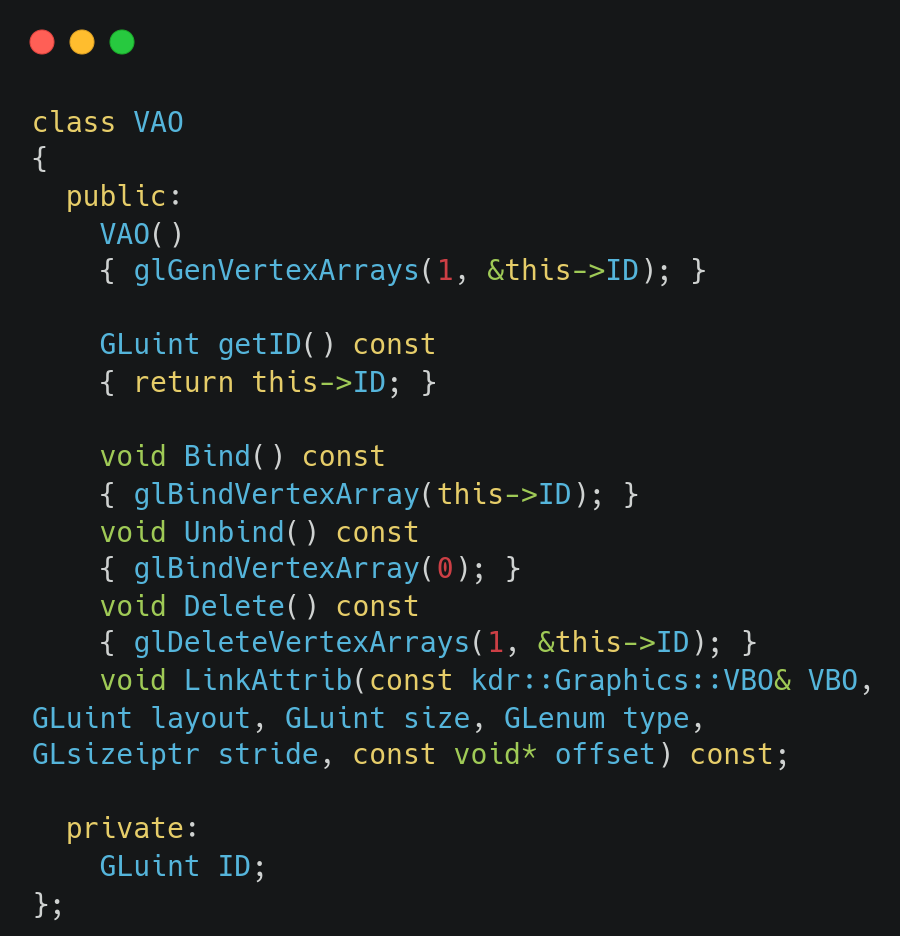
\includegraphics[height=10cm]{images/vao.png}
    \caption{Třída VAO}
    \label{fig:Třídy VAO}
\end{figure}

\pagebreak

Instance VAO mají své ID, metody \mintinline{cpp}{Use}, \mintinline{cpp}{Unbind} a \mintinline{cpp}{Delete}, navíc ale i metodu \mintinline{cpp}{LinkAttrib}. Ta jako své parametry vyžaduje odkaz na VBO, se kterým pracujeme, pořadí atributu, kolik hodnot zabírá atribut (např. 3 hodnoty), datový typ atributu, po kolika hodnotách se opakuje a kolik bytů je odsazen od začátku hodnot ve VBO. Jinak se se třídou VAO pracuje stejně, jako s třídami předchozími.

S použitím tříd VAO, VBO a EBO můžeme snadno využívat data o různorodých plochách a tělesech. Ať už jde o jednoduchý čtverec či komplexní model o řádech tisíců trojúhelníků. Pro představu, jak tyto třídy využívat nyní uvedu i příklad v kódu. Je ale nutné dodat, že proměnné \mintinline{cpp}{vrcholy}, \mintinline{cpp}{velikostVrcholu}, \mintinline{cpp}{indexy} a \mintinline{cpp}{velikostIndexu} musíme považovat, za již definované, neboť by jinak ukázka byla poměrně zdlouhavá a komplikující pochopení.

\vspace{0.5cm}
\begin{figure}[h]
    \centering
    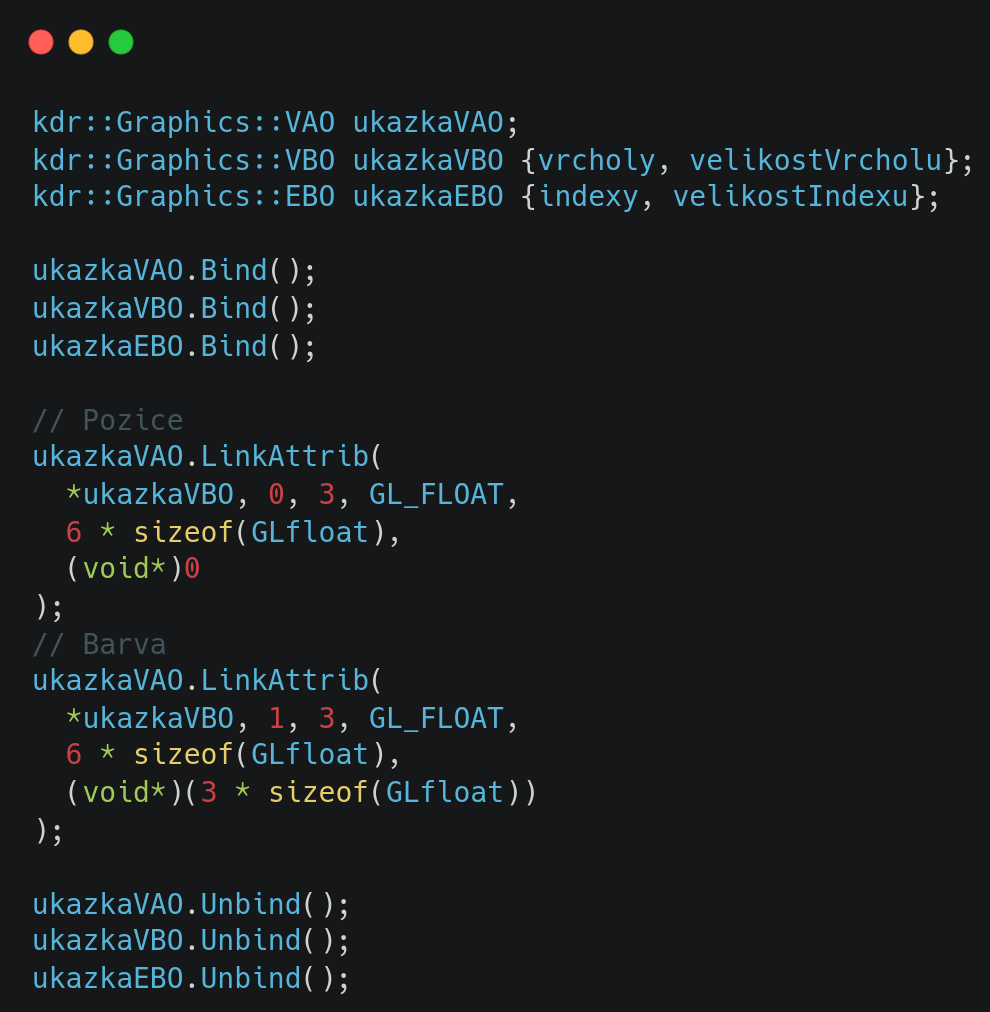
\includegraphics[height=11cm]{images/vao_vbo_ebo_example.png}
    \caption{Použití tříd VAO, VBO a EBO}
    \label{fig:Použití tříd VAO, VBO a EBO}
\end{figure}

\pagebreak

\subsection{Práce s prostorem}

Pro práci s prostorem jsem definoval několik tříd. Pro vektory jsou definovány třídy \mintinline{cpp}{Vec2} a \mintinline{cpp}{Vec3}. Z názvu lze usoudit, že první třída je pro vektor dvoudimenzionální, druhá pro vektor třídimenzionální. V praxi využívám 2D vektory při práci s pozicováním GUI na obrazovce. 3D vektory jsou využívány pro pozicování a pohyb s tělesy v prostoru. Další třídou je pak \mintinline{cpp}{Mat4}, představující matici s řádem $4 \times 4$. Jiné třídy nebylo potřeba definovat, neboť už jen tyto tři nám otevírají spoustu možností.

Pro vektory jsou definovány operace, které jsem popisoval i v kapitole \ref{vector} při analýze — sčítání, odčítání, násobení skalárem, skalární součin a vektorový součin (ten je definován jen pro třídu \mintinline{cpp}{Vec3}). U některých těchto funkcí využívám funkcionality C++, která se nazývá operator overloading. Ta nám umožňuje přidat speciální interakce třídám s existujícími operátory (+, -, +=, ...). Nemusím tak tvořit funkce či metody pro implementaci některých operací, mohu přidat interakce s existujícími operátory. \cite{operator_overloading} Třídu \mintinline{cpp}{Vec3} a overloading operátorů nyní představím na příkladu:

\vspace{0.5cm}
\begin{figure}[h]
    \centering
    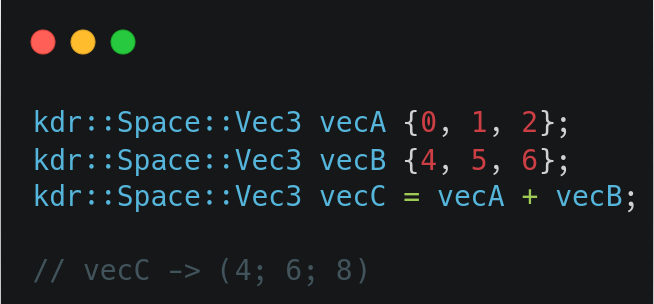
\includegraphics[height=4cm]{images/overloading.png}
    \caption{Třída Vec3 a její sčítání}
    \label{fig:Třída Vec3 a její sčítání}
\end{figure}

Jak vidíme na Obrázku \ref{fig:Třída Vec3 a její sčítání}, nevyužívám pro součet žádné metody či funkce. Kód je tak čitelnější a operace s vektory pak intuitivnější. Pro třídu \mintinline{cpp}{Mat4} je pak přidána funkcionalitě operátoru \mintinline{cpp}{[]}. Ten slouží pro získání hodnoty z pole. Bylo již zmíněno, že matice je souborem hodnot, který lze členit do řádek a sloupců. To se velmi nápadně podobá dvourozměrným polím. Problémem je, že \mintinline{cpp}{Mat4} je třída, takže pro získání hodnoty bychom standardně museli využívat funkcionality, která by mohla připomínat: \mintinline{cpp}{matice.getValue(1, 1)}, \mintinline{cpp}{matice.values[1][1]} či \mintinline{cpp}{matice.value(1, 1)}. Začnu představením, jak třída vypadá:

\pagebreak

\begin{figure}[h]
    \centering
    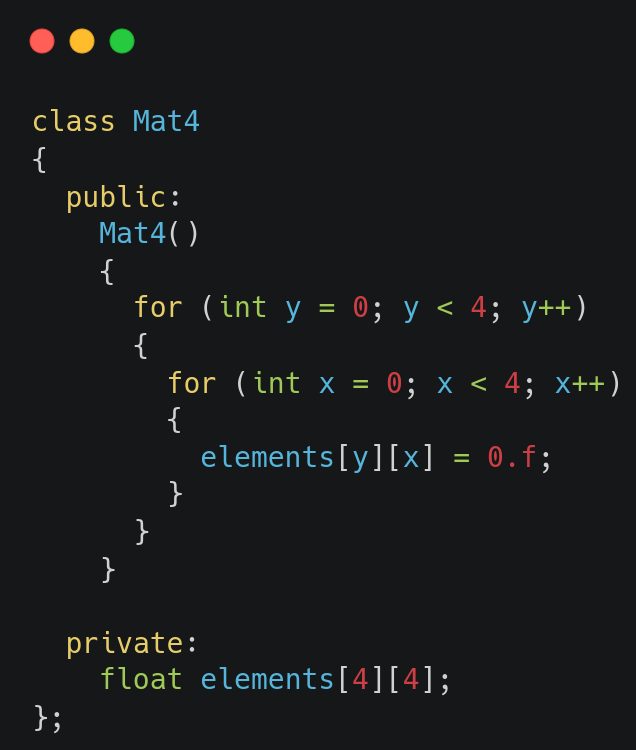
\includegraphics[height=8cm]{images/mat.png}
    \caption{Třída Mat4}
    \label{fig:Třída Mat4}
\end{figure}

\begin{figure}[!h]
    \centering
    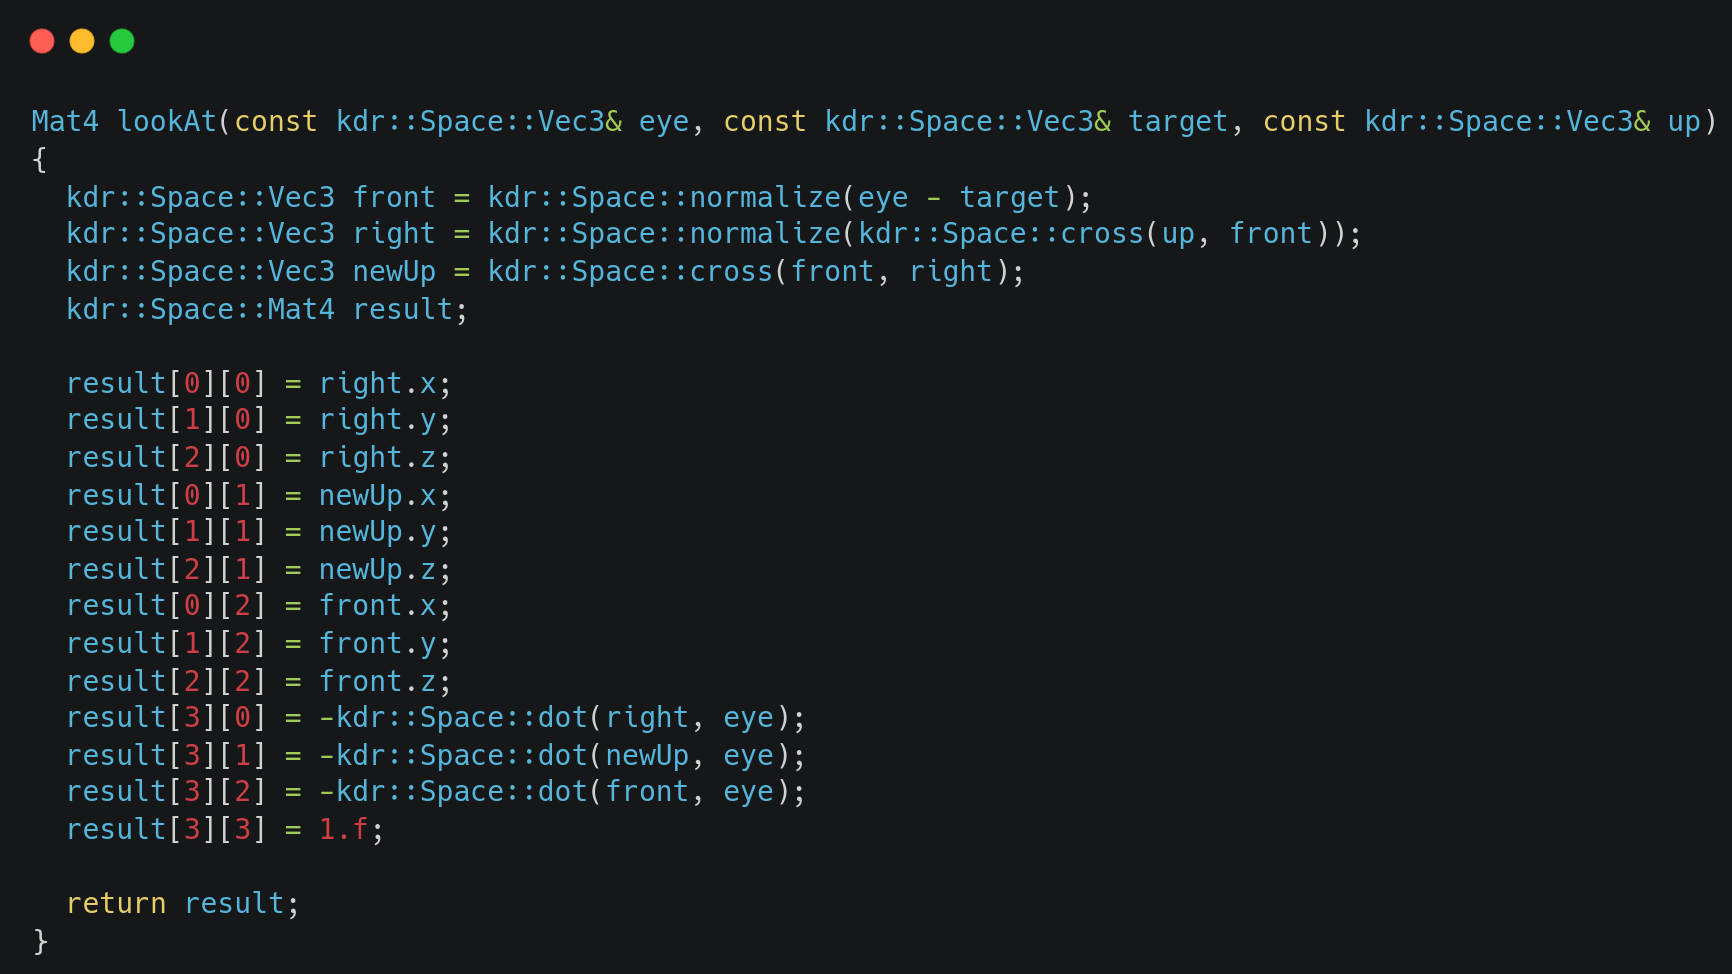
\includegraphics[height=8cm]{images/lookat_mat.png}
    \caption{Výpočet matice pro pohled kamery}
    \label{fig:Výpočet matice pro pohled kamery}
\end{figure}

\pagebreak

Jako první vidíme na obrázku \ref{fig:Třída Mat4} zjednodušenou třídu \mintinline{cpp}{Mat4}. Na Obrázku \ref{fig:Výpočet matice pro pohled kamery} pak vidíme využití trigonometrických funkcí a také funkce enginu pro výpočty skalárního a vektorového součinu. Výsledkem je matice, která nám popisuje pohled kamery daným směrem z dané pozice. Pomocí operator overloadingu mohu k prvkům matice přistupovat, jako bych přistupoval přímo k poli, tedy \mintinline{cpp}{matice[1][1]}. Je zde zastoupena i funkce pro normalizaci vektorů.

\subsection{Tělesa}

Engine také poskytuje vlastní třídy pro různá tělesa. Nejdůležitější třídou tohoto module je třída \mintinline{cpp}{Solid}, ze které všechna ostatní tělesa díky dědičnosti vycházejí. S~tělesy můžeme díky maticím a vektorům manipulovat, například posunem či rotací. Díky dědičnosti lze tyto operace provádět na všech dalších tělesech. Popis těles začnu uvedením minimalistické ukázky zmíněné třídy \mintinline{cpp}{Solid}:

\vspace{0.5cm}
\begin{figure}[!h]
    \centering
    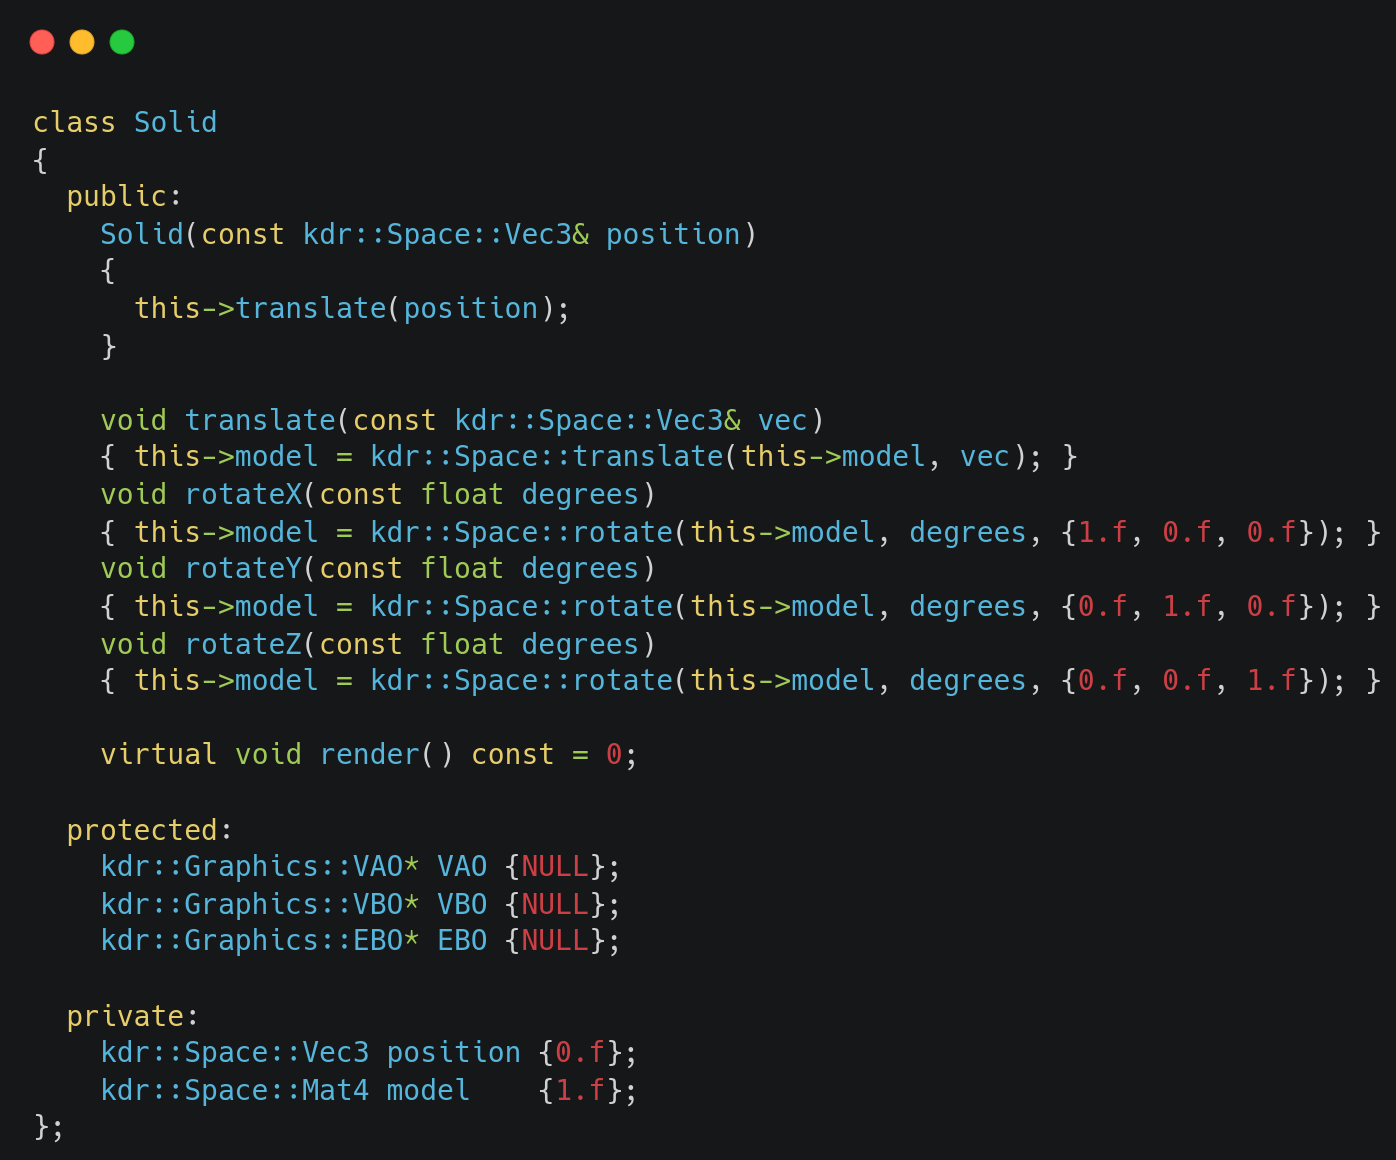
\includegraphics[height=9.5cm]{images/solid.png}
    \caption{Zjednodušená třída Solid}
    \label{fig:Zjednodušená třída Solid}
\end{figure}

Každé těleso má své VAO, VBO a EBO, jak lze vidět na obrázku \ref{fig:Zjednodušená třída Solid}. V enginu z této třídy vycházejí například třídy: \mintinline{cpp}{Cube}, \mintinline{cpp}{Cuboid}, \mintinline{cpp}{Pyramid} či \mintinline{cpp}{Mesh}, která slouží pro využívání vlastních modelů, jenž jsou čteny z Wavefront OBJ \cite{wavefront} souborů. Všechny data o vrcholech těles jsou ve stejném formátu — obsahují pozici, barvu vrcholu, souřadnice textury a normálový vektor pro bod.

\subsection{Uživatelské rozhraní}

Pro prvky uživatelského rozhraní je určen modul \mintinline{cpp}{GUI}. V něm se nachází třída \mintinline{cpp}{Element}. Tato třída je velmi podobná zmíněné třídě \mintinline{cpp}{Solid}. Má své VAO, VBO a EBO, pozici a metodu pro její vykreslení. Takto vypadá zjednodušený kód této třídy:

\vspace{0.5cm}
\begin{figure}[h]
    \centering
    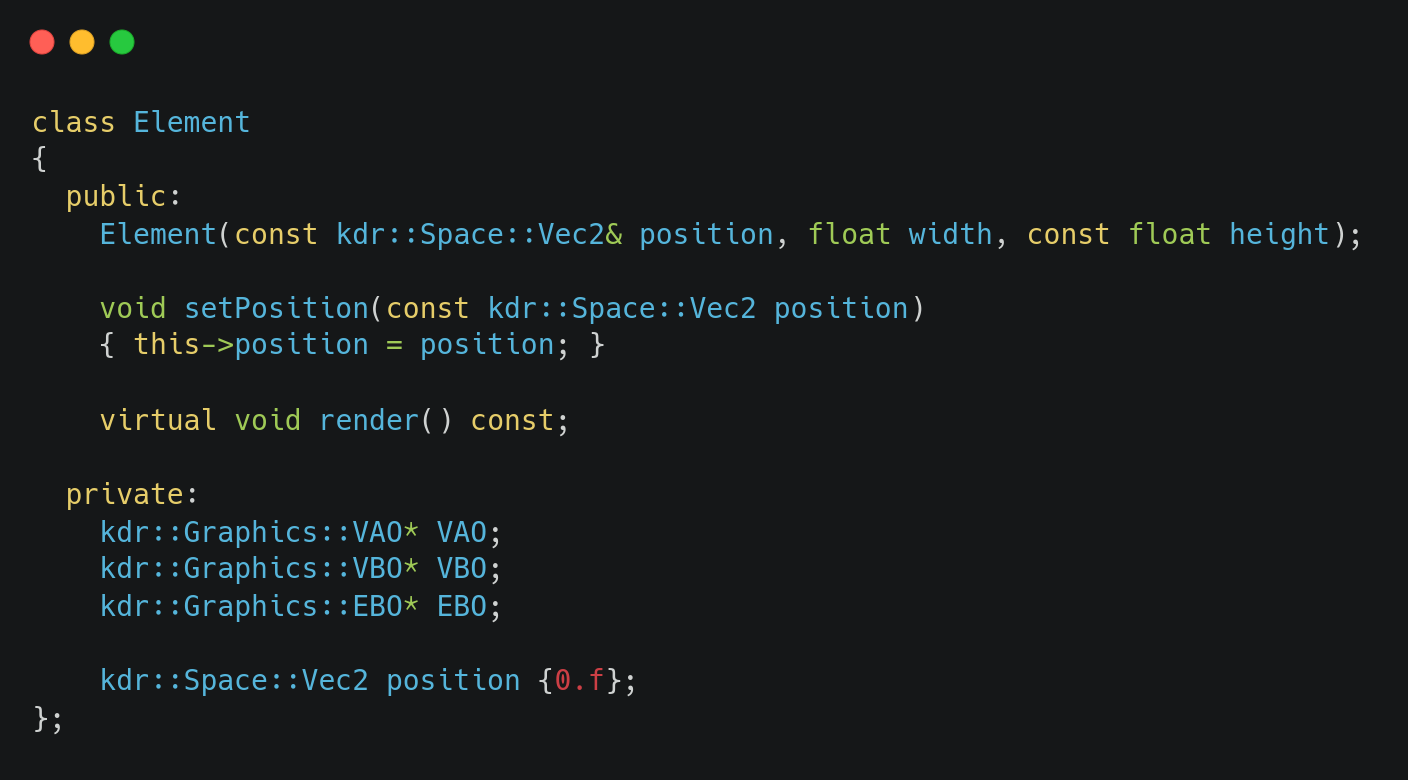
\includegraphics[height=7cm]{images/element.png}
    \caption{Třída Element}
    \label{fig:Třída Element}
\end{figure}

Z ní můžeme tvořit další třídy (např. pro lištu či ukazatel životů) nebo využívat přímo třídu \mintinline{cpp}{Element}. Na obrázku \ref{fig:Třída Element} vidíme, že narozdíl od třídy \mintinline{cpp}{Solid} však využívá dvoudimenzionální vektory a neobsahuje funkce pro rotaci. Informace o vrcholech obsahují méně informací, než u těles; konkrétně jde jen o pozici a souřadnice textury. V praxi využívám tuto třídu pro vytvoření crosshairu (mířítka ve středu obrazovky). Instance této třídy jsou cílené pro vykreslování ve 2D režimu, v případě omylného vykreslení ve 3D režimu se vykreslí jako plocha v prostoru.

\subsection{Světlo}

Pro světlo jsem vytvořil třídu \mintinline{cpp}{Light}, která popisuje barvu a pozici světla. Tato třída je určena k tomu, aby z ní byly vytvořené podtřídy, představující různé typy světla. Implementace aktuálně využívá pouze bodové světlo, které bylo vysvětleno v kapitole \ref{light} během analýzy. Zde je ukázka, jak třída \mintinline{cpp}{Light} vypadá:

\vspace{0.5cm}
\begin{figure}[h]
    \centering
    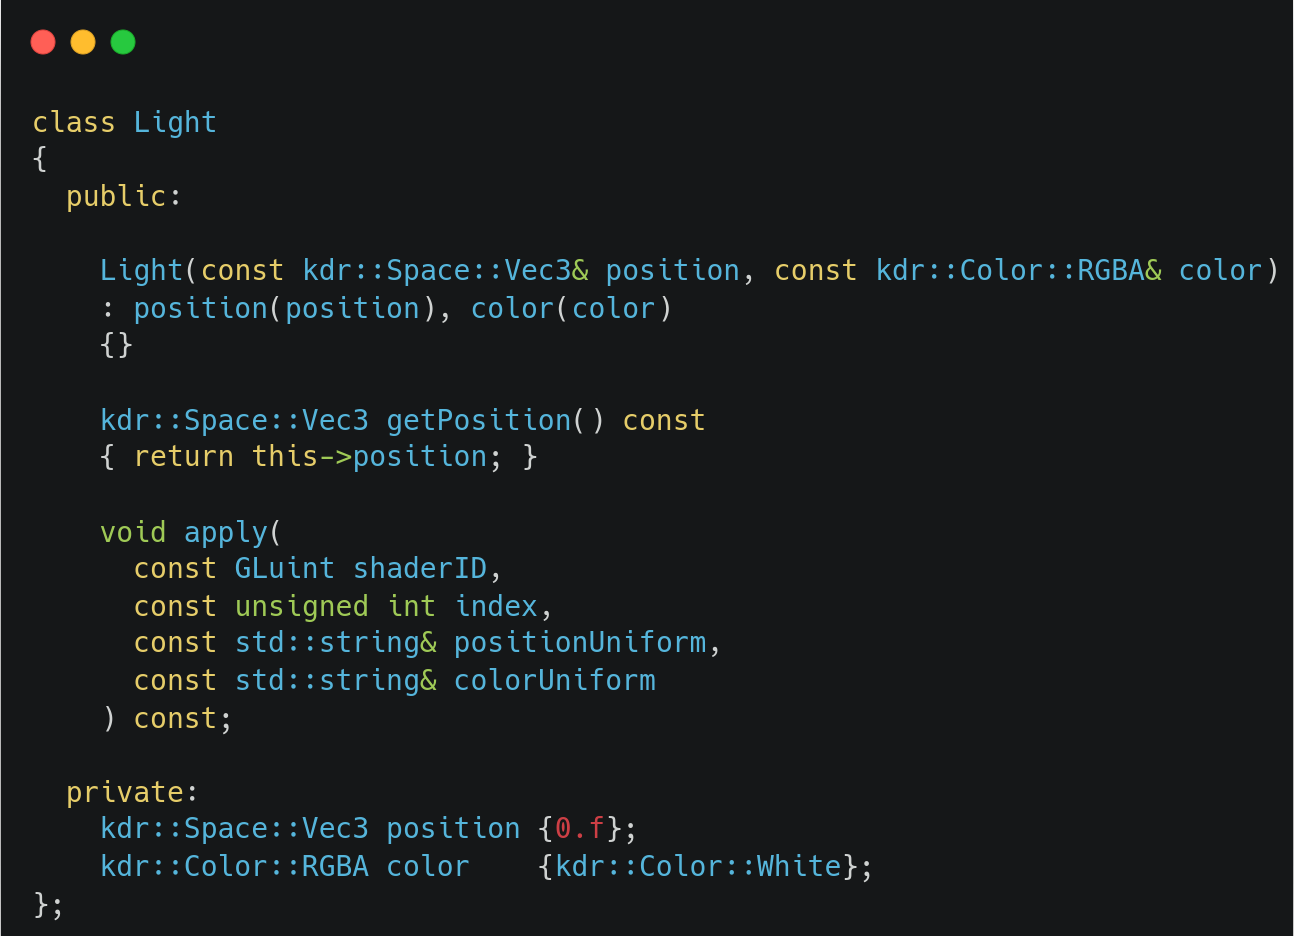
\includegraphics[height=7cm]{images/light.png}
    \caption{Třída Light}
    \label{fig:Třída Light}
\end{figure}

Tato třída, jak vidíme na Obrázku \ref{fig:Třída Light}, má svůj parametr pro barvu a pozici. Obsahuje také metodu, která umožňuje aplikovat světlo v shaderu a využívat ho tak při renderování.

\subsection{Čtení ze souborů}

Součástí enginu jsou také 2 moduly, které pracují se soubory. Jedná se o moduly \mintinline{cpp}{File} a \mintinline{cpp}{Image}. Jako první popíši, jak funguje modul \mintinline{cpp}{File}. Ten slouží pro získání obsahu jakéhokoliv souboru. Využívá se například pro čtení kódů pro shadery. Lze ho využít i pro jiné účely, dle potřeb programátora. Jedno z potencionálních využití by mohlo představovat čtení konfiguračních souborů. Funkce pro čtení souborů vypadá takto:

\vspace{0.5cm}
\begin{figure}[!h]
    \centering
    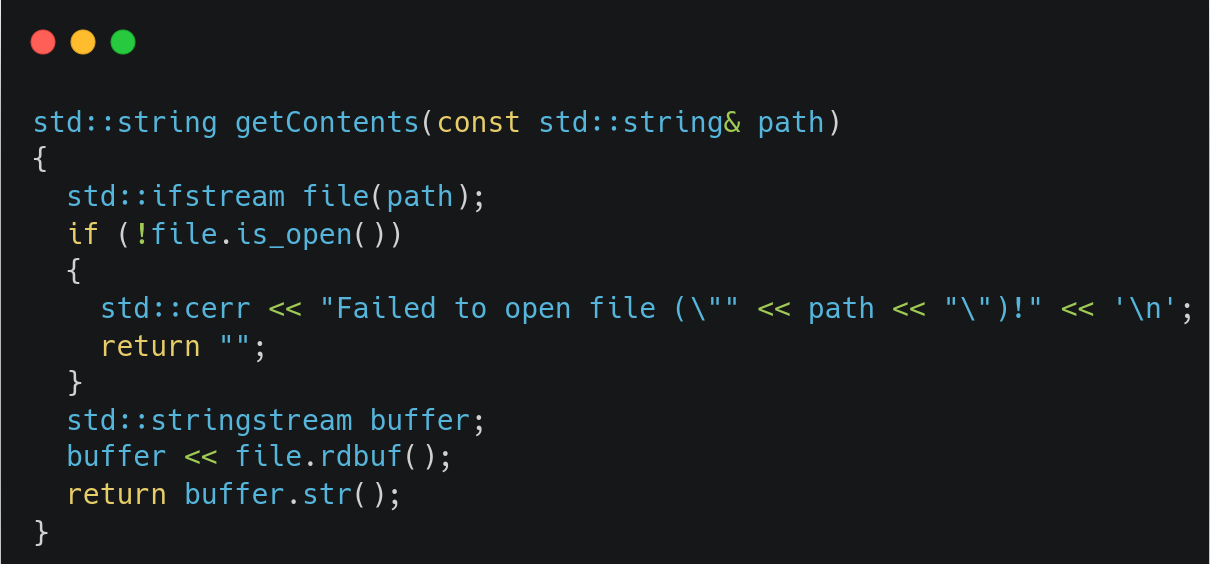
\includegraphics[height=6cm]{images/file.png}
    \caption{Funkce pro čtení souborů}
    \label{fig:Funkce pro čtení souborů}
\end{figure}

Funkce si jako parametr bere cestu k souboru, jenž chceme číst. Pokud soubor existuje, vrátí nám jeho obsah jako textový řetěz, v jiném případě pak vrací řetězec prázdný. Společně s prázdným řetězcem se pak do konzole vypíše chyba, že soubor s danou cestou k němu neexistuje.

Druhým modulem pro práci se soubory je modul \mintinline{cpp}{Image}. Ten slouží pro čtení souborů ve formátu PNG za pomocí knihovny libPNG. Získá nám data obrázku, jeho šířku, výšku a informaci o tom, zda obrázek obsahuje průhlednost. Náhled této funkce nebudu uvádět, neboť je poměrně rozsáhlá, obsahuje několik částí pro kontrolu chyb a také funkcí knihovny libPNG. Implementaci lze ale nalézt v souboru \mintinline{cpp}{/src/Image.cpp}.

\subsection{Integrace pro debugging}

Při práci s prostorem často potřebujeme vědět, s jakými daty aktuálně pracujeme nebo jaký je výsledek našich operací. Engine poskytuje modul \mintinline{cpp}{Debug}, který umožňuje vypsat si obsah vektoru či matice. Při testování a řešení problémů je to velmi užitečný nástroj, díky kterému vývojář nemusí řešit výpis hodnot sám. Takto vypadá využití funkce pro výpis matice:

\vspace{0.5cm}
\begin{figure}[!h]
    \centering
    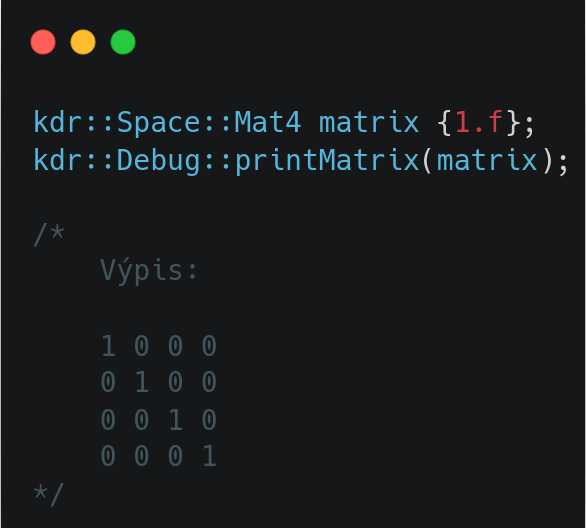
\includegraphics[height=5.5cm]{images/matrix_debug.png}
    \caption{Výpis obsahu matice}
    \label{fig:Výpis obsahu matice}
\end{figure}

Jak vidíme na Obrázku \ref{fig:Výpis obsahu matice} byla zvolena jednotková matice (ta má na diagonále všechny hodnoty rovné právě jedné). Podobná funkce je v enginu dostupná pod názvem \mintinline{cpp}{kdr::Debug::printVector}, která do jedná řádky vypíše složky vektoru.

\section{Uživatelská příručka}

V této sekci popisuji, jak kód budovat a spouštět na různých operačních systémech. Po vybudování ukázkového příkladu můžeme engine otestovat. Ovládání ukázkového příkladu je následovné:

\begin{enumerate}
    \item E - zamkne myš, můžeme tak otáčet a hýbat kamerou
    \item Escape - odemkne myš
    \item C - změní zobrazovací režim na body
    \item V - změní zobrazovací režim na hrany
    \item B - změní zobrazovací režim na plochy
    \item WSAD - pohyb v prostoru
    \item F - zapnutí a vypnutí fullscreen režimu
\end{enumerate}

\subsection{Linux}

Pro spuštění a vybudování kódu na operačním systému Linux budeme potřebovat několik balíčků na našem systému. S vysokou pravděpodobností nástroj \mintinline{bash}{make} již máme na systému nainstalován, přesto ho uvedu do instalačních příkazů. Dále budeme potřebovat nástroj CMake, který byl v práci již popsán. Na systému musí být rovněž nainstalován C++ compiler, např. g++. Jejich instalace se liší na bázi distribuce Linuxu, zde ale uvádím příkazy pro nejčastější distribuce:

\noindent\textbf{Debian/Ubuntu}:\\
\mintinline{bash}{sudo apt install cmake make g++}

\noindent\textbf{Fedora}:\\
\mintinline{bash}{sudo dnf install cmake make gcc-c++}

\noindent\textbf{Arch/Manjaro}:\\
\mintinline{bash}{sudo pacman -S cmake make gcc}

Máme-li tyto nástroje, můžeme v kořenovém adresáři přidat povolení budovacího skriptu. Pokud jsme vše provedli správně, vytvoří se nám spustitelná aplikace na této cestě (vůči kořenovému adresáři projektu): \mintinline{bash}{./build/examples/example}. Proces buildu a spuštění vypadá takto:

\vspace{0.5cm}
\begin{figure}[!h]
    \centering
    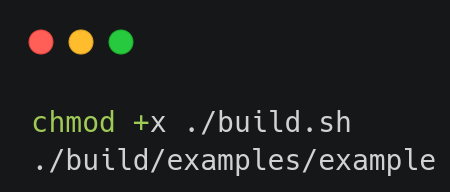
\includegraphics[height=3.5cm]{images/build.png}
    \caption{Vybudování a spuštění aplikace}
    \label{fig:Vybudování a spuštění aplikace}
\end{figure}

\subsection{Windows}

Pro kompilaci a budování přímo pro plaformu Windows aktuálně není návod, neboť Windows vyžaduje bez využití platformy Visual Studio a pouze CMake komplikované linkování DLL souborů. To ale neznamená, že kód na Windows nelze spustit a budovat. Můžeme si stáhnout WSL (Windows Subsystem For Linux) a používat tak Windows, jako bychom využívali nějakou Linuxovou distribuci. Pak je proces stejný, jako při budování na Linuxu.

Microsoft poskytuje oficiální návod, jak WSL instalovat a využívat na tomto odkazu:
\mintinline{bash}{https://learn.microsoft.com/en-us/windows/wsl/install}

\subsection{MacOS}

Kompilace na MacOS je velice podobná, jako kompilace na Linuxu; obojí jsou to totiž *NIX systémy. Stejně jako u Linuxu se musíme ujistit, že na systému jsou instalovány balíčky potřebné pro kompilaci. MacOS má svůj vlastní manager balíčků, který se nazývá Homebrew. Potřebné balíčky nainstalujeme takto:

\noindent\mintinline{bash}{sudo brew install make cmake gcc glew glfw libpng}

Dále je nutné nastavit některé proměnné prostředí (máte-li Homebrew nainstalován jinde, je třeba cestu k němu zaměnit):

\noindent\mintinline{bash}{export CPATH=/opt/homebrew/include}\\
\noindent\mintinline{bash}{export LIBRARY_PATH=/opt/homebrew/lib}

Následně je proces identický, jako pro platformu Linux. Uděláme buildovací skript spustitelným, spustíme ho a aplikaci najdeme na stejné cestě, jako na Linuxu.

\pagebreak

\section{Závěr}

Vytvořil jsem engine, který abstrahuje práci s grafickými koncepty. Umožňuje vývoj pro více platforem a nabízí tak vývojářům jednoduchý nástroj pro tvorbu her, animací či různých vizualizací. Díky tomu, že je kód důsledně komentován a funkce jsou systematicky pojmenovávány, je práce snadno rozšiřitelná. Jednotlivé metody a funkce jsou systematicky pojmenovávány a tak i snadno pochopitelné.

Zmíněnými rozšířeními by mohla být implementace více typů světel, podpora vykreslování textu na obrazovku či načítání scén ze souboru. Moderní hardware nám dává základ pro vývoj velmi pokročilých aplikací; umožňuje nám ale i snáze tolerovat nevýkonnost aplikací. Rozdíl v jednotkách desítek či stovek MB využití v paměti jsou dnes poměrně zanedbatelné, několik desítek let zpět by se ale jednalo o extrémní skok. Jako další zlepšení bych také uvedl lepší kompilaci na systému Windows a distribuci .exe souborů.

Práce může posloužit rovněž také pro zamyšlení, zda pro jednoduché hry potřebujeme používat profesionální herní enginy, ve kterých vyvíjí komplexní hry velká studia o stovkách vývojářů. Engine šetří desítky hodin programátorů, které by musely trávit studiem grafických rozhraní a následnou implementací, přičemž jim neříká, jak implementovat logiku a řešení svého problému.

Mně osobně engine dal také mnoho zkušeností se správou kódu a prohloubil mé znalosti matematiky. Konkrétně mi výrazně pomohl pochopit spojitosti při práci s prostorem v rámci lineární algebry. Tvorbu enginu bych doporučil každému, kdo chce lépe chápat strukturování dat či vidět, jak matematiku lze aplikovat v praxi.

Práci považuji za úspěšnou a obohacující jak pro ostatní vývojáře, tak pro mě samotného. Byla vytvořena funkční, minimalistická alternativa pro komerční řešení. Cíl práce byl tedy splněn. Zdrojový kód je dostupný pod open-source licencí GNU GPLv3 na portál GitHub. Projekt lze nalézt na odkaze: \\\mintinline{bash}{https://github.com/marcothelost/kedarium}.

\pagebreak

\section{Seznam použité literatury}

\printbibliography[heading=none]

\pagebreak

\section{Seznam obrázků a tabulek}

\listoffigures

\end{document}
